% !TeX document-id = {b4ed2942-570a-4bca-8c62-e711ae21c729}
% !TeX TXS-program:compile = txs:///pdflatex/
% !BIB program = biber



\documentclass[aspectratio=169, 11pt, t]{beamer}

% !TeX TXS-program:compile = txs:///pdflatex/
% !BIB program = biber




%%%%%%%%%%%%%%%%%%%%%%%%%%%%
%%  FUNDAMENTAL SETTINGS  %%
%%%%%%%%%%%%%%%%%%%%%%%%%%%%


\newcommand{\serifbodyfont}{0}
% 0: Body is set in sans-serif font
% 1: Body is set in serif font
\newcommand{\serifheadingfont}{0}
% 0: Headings (``structure'') are set in sans-serif font
% 1: Headings (``structure'') are set in serif font

\newcommand{\showsectionnavigation}{0}
% 0: ``Headline'' is disabled.
% 1: ``Headline'' (at the very top of slides) is included and displays all sections of the presentation,
%      with the current section being highlighted.




%%%%%%%%%%%%%%%%%%%%%%%%%%%%
%%  FUNDAMENTAL PACKAGES  %%
%%%%%%%%%%%%%%%%%%%%%%%%%%%%


\usepackage{ifthen}

\usepackage{calc}

\usepackage{tcolorbox}

\usepackage[LY1, LGR, TS1, T1]{fontenc}
% LGR (Greek) is needed to enable the ``sansserif math'' features.
\usepackage[utf8]{inputenc}

\usepackage{tabularx}

\ifxetex
\usepackage[protrusion=true, expansion=false]{microtype}
\else
\usepackage[protrusion=true, expansion=false, kerning=true]{microtype}
\fi
% The microtype package enables so-called hanging punctuation. That is, when a punctuation sign like ":", ".", "-", etc. is found at the beginning or end of a line, it is protruded a little into the page margin. This results in "optical margin alignment," because the protrusion makes the margin alignment look straighter.


\definecolor{darkgray}{rgb}{0.4,0.4,0.4}

\usepackage[absolute, overlay]{textpos}
\usepackage{graphicx}
\usepackage{amsmath}
%\usepackage{amsfonts}
%\usepackage{amssymb}
\usepackage{epstopdf}
\DeclareGraphicsRule{.tif}{png}{.png}{`convert #1 `dirname #1`/`basename #1 .tif`.png}

\usepackage[ngerman, american, USenglish]{babel}
% German and US English hyphenation and quotation marks
\selectlanguage{USenglish}
\usepackage[autostyle=true]{csquotes}

\usepackage{multirow}

\usepackage{xcolor}
\usepackage{pgf}%,pgfarrows,pgfnodes,pgfshade}
\usepackage{tikz}
\usepackage{pgfplots}
\usetikzlibrary{mindmap, trees, patterns, arrows.meta}

\usepackage{xspace}

% \usepackage{eurosym}

%\usepackage{etoolbox}
%	% Enables manipulating LaTeX commmands via \preto, \appto, \patchcmd, etc.
%	% loaded automatically by beamer
\usepackage{xpatch}
% Enables manipulating LaTeX commmands via \xpatchcmd etc.

\hypersetup{%
	colorlinks, linkcolor=, urlcolor=SpotColor, citecolor=%
}
\urlstyle{same}
\newcommand{\email}[1]{\href{mailto:#1}{\nolinkurl{#1}}}




%%%%%%%%%%%%%%%%%%%%%
%%  FONT SETTINGS  %%
%%%%%%%%%%%%%%%%%%%%%


% !TeX TXS-program:compile = txs:///pdflatex/
% !TeX TS-program = pdflatex
% !TeX TXS-program:bibliography = txs:///biber
% !BIB program = biber




%%%%%%%%%%%%%%%%%%%%%%%%%%%%%%%%%%%%
%%  FONT SETTINGS AND TYPOGRAPHY  %%
%%%%%%%%%%%%%%%%%%%%%%%%%%%%%%%%%%%%


% Use Fira Sans as the sans-serif font.
% Load first because it otherwise doesn't work properly.
% ==>
%\usepackage[lining, scale=0.88]{FiraMono}  % To match the x-height of the Charter serif font
%\usepackage[book, semibold, lining, tabular, scale=0.88]{FiraSans}[2018/05/23]
%\makeatletter
%\@ifpackagelater{FiraSans}{2018/05/23}
%	{}
%	{\PackageError{FiraSans}
%	     {Outdated 'FiraSans' package}
%	     {Upgrade to FiraSans 2018/05/23 or newer!\MessageBreak
%	      Otherwise the sans-serif font may not work properly, or the compilation might fail.\MessageBreak
%	      This is a fatal error. I'm aborting now.}%
%	\endinput%
%   }
%\makeatother
%% In case you wish to use the ``light'' options of FiraSans: -->
%\ifthenelse{\isundefined{\AfterPackage}}{\usepackage{afterpackage}}{}
%\AfterPackage{siunitx}{%
%  \providecommand*{\lseries}{\fontseries{l}\selectfont}
%}
% See https://tex.stackexchange.com/questions/164791/combination-of-siunitx-and-light-weight-font-fails-to-compile.
% <--
% <==

\usepackage[xcharter, slantedGreek, scaled=1.09]{newtxmath}
% This template also works with the ``IBM Plex Sans'' and ``IBM Plex Mono'' fonts,
% https://ctan.org/pkg/plex ==>
\usepackage[semibold, scale=0.94]{plex-mono}  % To match the x-height of the Charter serif font
\usepackage[textmd, semibold, scale=0.94]{plex-sans}[2018/12/31]
% Earlier versions of the ``plex-sans'' package do not include support for LGR Greek.
% <==

%% This template also works with the ``Alegreya'' and ``Alegreya Sans'' fonts,
%% https://ctan.org/pkg/alegreya ==>
%\usepackage[semibold, scale=0.89]{plex-mono}  % To match the x-height of the Charter serif font
%\usepackage[lining, tabular, scale=1.02]{AlegreyaSans}[2018/08/02]
%	% Earlier versions of the ``Alegreya'' package do not include support for LGR Greek.
%% <==

%% This template also works with the ``Google Noto'' fonts,
%% https://ctan.org/pkg/noto ==>
%\usepackage[scale=0.85]{noto-mono}
%\usepackage[lining, tabular, scale=0.85]{noto-sans}[2019/01/11]
%	% Earlier versions of the ``noto'' package do not include support for LGR Greek.
%% <==

% Save the font family and font series definitions for later use: ==>
\newcommand{\savesffamily}{\sfdefault}
\makeatletter
\newcommand{\savesfmdseries}{\mdseries@sf}
\newcommand{\savesfbfseries}{\bfseries@sf}
\makeatother
% <==

% Use Bitstream Charter as the math font
% ==>
%\usepackage[charter, greeklowercase=italicized, greekuppercase=italicized, sfscaled=false, ttscaled=false]{mathdesign}
%% Use Alegreya as the text font -->
%\usepackage[lining, tabular, scale=1.02]{Alegreya}[2018/08/02]
%\ifxetex \else \DisableLigatures[T]{family = {rm*}} \fi
%% <--
%% Use Noto Serif as the text font -->
%\usepackage[lining, tabular, scale=0.85]{noto-serif}[2019/01/11]
%% <--
% Use IBM Plex as the text font -->
\usepackage[textmd, semibold, scale=0.94]{plex-serif}
% <--
% Save the font family and font series definitions for later use:
\let \savermfamily \rmdefault
\makeatletter
\newcommand{\savermmdseries}{\mdseries@rm}
\newcommand{\savermbfseries}{\bfseries@rm}
\makeatother
% <==

% mathdesign provides upright Greek letters as \alphaup, \Betaup, etc. while other packages
% (e.g., unicode-math) call these \upalpha, \upBeta, etc. We make also the latter available.
% ==>
\makeatletter
\@for\@tempa:=%
	alpha,beta,gamma,delta,epsilon,zeta,eta,theta,iota,kappa,lambda,mu,nu,xi,%
	omicron,pi,rho,sigma,varsigma,tau,upsilon,phi,chi,psi,omega,digamma,%
	Alpha,Beta,Gamma,Delta,Epsilon,Zeta,Eta,Theta,Iota,Kappa,Lambda,Mu,Nu,Xi,%
	Omicron,Pi,Rho,Sigma,Tau,Upsilon,Phi,Chi,Psi,Omega,Digamma%
\do{%
	\expandafter\let\csname up\@tempa\expandafter\endcsname\csname\@tempa up\endcsname%
}%
\makeatother
% <==

% Provide a \nequiv symbol
\ifx\nequiv\undefined
	\newcommand{\nequiv}{\not\equiv}
\fi

% Use Bitstream Charter as the text font
% ==>
%\usepackage[scaled=.96, lining, sups]{XCharter}  % option ``sups'' not working properly with subimport
% Save the font family and font series definitions for later use:
\let \savermdefaultfortext \rmdefault
\let \savemddefaultfortext \mddefault
\let \savebfdefaultfortext \bfdefault
\renewcommand{\textellipsis}{\mbox{.{\kern.09em}.{\kern.09em}.}}
%\makeatletter
%\newcommand{\@makefnmarkorig}{%
%	\hbox{\sufigures\hspace*{.04em}\@thefnmark\hspace*{.04em}}%
%}  % Copied from XCharter.sty
%\makeatother
% <==

\ifxetex
	% Do nothing.
\else
	\DisableLigatures[f]{family = {rm*, tt*}}
	% Disable the f* ligatures for Charter because the font does not provide sufficient support.
	% Disable the f* ligatures for the ``typewriter'' font because they make no sense for a monospaced font.
	\SetExtraKerning[unit=space]
		{encoding=*, family=*, series=*, size={*, normalsize, footnotesize}, font = */*/*/*/*}
		{\textemdash = {325, 325},
			/ = {100, 100},
			: = { 50,   0},
			; = { 50,   0}}
\fi

\usepackage{xfrac}	% Provides \sfrac

% Since math mode uses a different font encoding, issuing \euro/\texteuro in math mode
% produces an incorrect sign. We fix this. ==>
\AtBeginDocument{%
	\providecommand{\euro}[1]{%
		\relax\ifmmode\text{\texteuro}#1\else\texteuro #1\fi%
	}%
}
% <==

\ifnum \serifbodyfont=0
	\setbeamerfont{normal text}{family=\sffamily}
	\renewcommand{\familydefault}{\savesffamily}
	\renewcommand{\rmdefault}{\savesffamily}
	\renewcommand{\mddefault}{\savesfmdseries}
	\renewcommand{\bfdefault}{\savesfbfseries}
	\AtBeginDocument{\sffamily}
\else
	\usefonttheme{serif}
	\setbeamerfont{normal text}{family=\rmfamily}
\fi
\ifnum \serifheadingfont=0
	\setbeamerfont{structure}{family=\sffamily, shape=\upshape, series=\bfseries}
\else
	\setbeamerfont{structure}{family=\rmfamily, shape=\upshape, series=\bfseries}
\fi

% Make frame titles and headings bold
\usefonttheme{structurebold}
\usefonttheme{professionalfonts}

\ifnum \serifheadingfont=0
	\setbeamerfont{footline}
		{parent=structure, size=\tiny, series=\mdseries}
\else
	\setbeamerfont{footline}
		{parent=structure, size=\tiny, series=\fontseries{\savermmdseries}}
\fi
\setbeamercolor{footline}
	{fg=SpotColor}

%% Use the bm (= boldmath) package for better support of setting math in bold ==>
%% Prevent the "Too many math fonts used" error:
\newcommand{\bmmax}{0}
\newcommand{\hmmax}{0}
\usepackage{bm}
%% <==

\usepackage{fontawesome}

\usepackage{mathtools}
%\mathtoolsset{centercolon}
% This makes the compilation fail in combination with tikz. See
% https://tex.stackexchange.com/questions/89467/why-does-pdftex-hang-on-this-file.
%% Inspired by https://tex.stackexchange.com/questions/251460/how-to-put-symbols-of-equal-size-on-top-of-each-other
%\newcommand{\succeqq}{%
%	\mathrel{%
%		\vcenter{\offinterlineskip
%			\ialign{##\cr$\succ$\cr\noalign{\kern 1pt}$=$\cr}%
%		}%
%	}%
%}
%\newcommand{\nsucceqq}{\mathrel{\not\succeqq}}
%\newcommand*{\coloneqq}{\mathrel{%
%		\mathrel{%
%			\raisebox{0.15ex}{\scalebox{0.85}{\ensuremath{:}}}\hspace{-0.2pt}%
%		}%
%		=%
%}}

% !TeX TXS-program:compile = txs:///pdflatex/
% !TeX program = pdflatex




%%%%%%%%%%%%%%%%%%%%%%%%%%%%%%%%%%%%%%%%%%%%%%%%%
%%  SANS-SERIF MATH IN SANS-SERIF ENVIRONMENT  %%
%%%%%%%%%%%%%%%%%%%%%%%%%%%%%%%%%%%%%%%%%%%%%%%%%


% See https://tex.stackexchange.com/questions/41497/how-to-typeset-some-text-including-math-content-in-sans-serif
% See https://tex.stackexchange.com/questions/33165/make-mathfont-respect-the-surrounding-family

% Necessary for use of kpfonts
% ==>
\makeatletter
\newif\ifkp@upRm
\newif\ifkp@osm
\newif\ifkp@vosm
\makeatother
% <==

\DeclareMathVersion{normalup}
\DeclareMathVersion{boldup}
\DeclareMathVersion{sans}

%\SetSymbolFont{operators}{sans}{OT1}{jkpss}{m}{n}
%	% From http://mirrors.ctan.org/fonts/kpfonts/latex/kpfonts.sty
\SetSymbolFont{operators}   {sans}{OT1}{mdbch}{m}{n}
\SetSymbolFont{letters}     {sans}{OML}{jkpss}{m}{it}
	% From http://mirrors.ctan.org/fonts/kpfonts/latex/kpfonts.sty
%\SetSymbolFont{letters}     {sans}{OML}{cmbrm}{m}{it}
%\SetSymbolFont{symbols}     {sans}{OMS}{cmbrs}{m}{n}
\SetSymbolFont{symbols}     {sans}{OMS}{jkp}  {m}{n}
	% From http://mirrors.ctan.org/fonts/kpfonts/latex/kpfonts.sty
\DeclareSymbolFont{extrasymbols}  {OMS}{cmbrs}{m}{n}
\SetSymbolFont{extrasymbols}{sans}{OMS}{cmbrs}{m}{n}
	% Some symbols (e.g., \prime) look weird in kpfonts.
	% This provides the option to replace them by symbols from mathdesign-charter.

\SetMathAlphabet{\mathit} {sans}{OT1}{\savesffamily}{\savesfmdseries}{it}
\SetMathAlphabet{\mathbf} {sans}{OT1}{\savesffamily}{\savesfbfseries}{n}
\SetMathAlphabet{\mathtt} {sans}{OT1}{cmtl}{m}{n}
\SetMathAlphabet{\mathcal}{sans}{OMS}{ntxsy}{m}{n}
	% See https://tex.stackexchange.com/questions/231583/import-mathcal-symbols-from-txfonts
%\SetSymbolFont{largesymbols}{sans}{OMX}{jkpss}{m}{n}
%	% From http://mirrors.ctan.org/fonts/kpfonts/latex/kpfonts.sty
\SetSymbolFont{largesymbols} {sans}{OMX}{mdbch}{m}{n}
	% Using symbols like \int, \left(, etc. from mathdesign-charter because they look better than the ones included in kpfonts

\DeclareMathVersion{sansup}
\SetSymbolFont{letters}  {sansup}{OML}{jkpss}{m}{it}
\SetSymbolFont{symbols}  {sansup}{OMS}{jkp}  {m}{n}

\DeclareMathVersion{boldsans}
%\SetSymbolFont{operators}{boldsans}{OT1}{jkpss}{b}{n}
%	% From http://mirrors.ctan.org/fonts/kpfonts/latex/kpfonts.sty
\SetSymbolFont{operators}{boldsans}{OT1}{mdbch}{bx}{n}
\SetSymbolFont{letters}  {boldsans}{OML}{jkpss}{bx}{it}
	% From http://mirrors.ctan.org/fonts/kpfonts/latex/kpfonts.sty
%\SetSymbolFont{letters}  {boldsans}{OML}{mdbch}{bx}{it}
%\SetSymbolFont{letters}{boldsans}{OML}{cmbrm}{b}{it}
\SetSymbolFont{symbols}  {boldsans}{OMS}{jkp}  {bx}{n}
	% From http://mirrors.ctan.org/fonts/kpfonts/latex/kpfonts.sty
%\SetMathAlphabet{\mathrm}{boldsans}{OT1}{\savesffamily}{\savesfbfseries}{n}
\SetMathAlphabet{\mathit} {boldsans}{OT1}{\savesffamily}{\savesfbfseries}{it}
\SetMathAlphabet{\mathtt} {boldsans}{OT1}{cmtl}{b}{n}
\SetMathAlphabet{\mathcal}{boldsans}{OMS}{ntxsy}{b}{n}
%\SetSymbolFont{largesymbols}{boldsans}{OMX}{jkpss}{bx}{n}
%	% From http://mirrors.ctan.org/fonts/kpfonts/latex/kpfonts.sty
\SetSymbolFont{largesymbols}{boldsans}{OMX}{mdbch}{bx}{n}
	% Using symbols like \int, \left(, etc. from mathdesign-charter because they look better than the ones included in kpfonts

\DeclareMathVersion{boldsansup}
%\SetSymbolFont{letters}{boldsansup}{OML}{jkpss}{bx}{it}
%SetSymbolFont{symbols}{boldsansup}{OMS}{jkp}  {bx}{n}

% Using glyphs for math mode from the custom sansserif font
%\DeclareSymbolFont{uprightglyphs}{T1}{\savermfamily}{\savermmdseries}{n}
%\SetSymbolFont{uprightglyphs}{normal}    {T1}{\savermfamily}{\savermmdseries}{n}
%\SetSymbolFont{uprightglyphs}{normalup}  {T1}{\savermfamily}{\savermmdseries}{n}
%\SetSymbolFont{uprightglyphs}{bold}      {T1}{\savermfamily}{\savermbfseries}{n}
%\SetSymbolFont{uprightglyphs}{boldup}    {T1}{\savermfamily}{\savermbfseries}{n}
%\SetSymbolFont{uprightglyphs}{sans}      {T1}{\savesffamily}{\savesfmdseries}{n}
%\SetSymbolFont{uprightglyphs}{sansup}    {T1}{\savesffamily}{\savesfmdseries}{n}
%\SetSymbolFont{uprightglyphs}{boldsans}  {T1}{\savesffamily}{\savesfbfseries}{n}
%\SetSymbolFont{uprightglyphs}{boldsansup}{T1}{\savesffamily}{\savesfbfseries}{n}
%\DeclareSymbolFont{italicglyphs} {T1}{\savermfamily}{\savermmdseries}{it}
%\SetSymbolFont{italicglyphs} {normal}    {T1}{\savermfamily}{\savermmdseries}{it}
%\SetSymbolFont{italicglyphs} {normalup}  {T1}{\savermfamily}{\savermmdseries}{n}
%\SetSymbolFont{italicglyphs} {bold}      {T1}{\savermfamily}{\savermbfseries}{it}
%\SetSymbolFont{italicglyphs} {boldup}    {T1}{\savermfamily}{\savermbfseries}{n}
%\SetSymbolFont{italicglyphs} {sans}      {T1}{\savesffamily}{\savesfmdseries}{it}
%\SetSymbolFont{italicglyphs} {sansup}    {T1}{\savesffamily}{\savesfmdseries}{n}
%\SetSymbolFont{italicglyphs} {boldsans}  {T1}{\savesffamily}{\savesfbfseries}{it}
%\SetSymbolFont{italicglyphs} {boldsansup}{T1}{\savesffamily}{\savesfbfseries}{n}

% Syntax of \DeclareMathSymobl:
% \DeclareMathSymbol {<symbol>} {<type>} {<sym-font>} {<slot>}
% Type              Meaning	            Example
% 0 or \mathord     Ordinary             $\alpha$
% 1 or \mathop      Large operator       $\sum$
% 2 or \mathbin     Binary operation     $\times$
% 3 or \mathrel     Relation             $\leq$
% 4 or \mathopen    Opening              $\langle$
% 5 or \mathclose   Closing              $\rangle$
% 6 or \mathpunct   Punctuation          ;
% 7 or \mathalpha   Alphabet character   A
% Example declaration:
% \DeclareMathSymbol{b}{0}{letters}{`b}

% Digits
%\DeclareMathSymbol{0}{\mathalpha}{uprightglyphs}{`0}
%\DeclareMathSymbol{1}{\mathalpha}{uprightglyphs}{`1}
%\DeclareMathSymbol{2}{\mathalpha}{uprightglyphs}{`2}
%\DeclareMathSymbol{3}{\mathalpha}{uprightglyphs}{`3}
%\DeclareMathSymbol{4}{\mathalpha}{uprightglyphs}{`4}
%\DeclareMathSymbol{5}{\mathalpha}{uprightglyphs}{`5}
%\DeclareMathSymbol{6}{\mathalpha}{uprightglyphs}{`6}
%\DeclareMathSymbol{7}{\mathalpha}{uprightglyphs}{`7}
%\DeclareMathSymbol{8}{\mathalpha}{uprightglyphs}{`8}
%\DeclareMathSymbol{9}{\mathalpha}{uprightglyphs}{`9}
% Operators and punctuation
\DeclareMathSymbol{+}{\mathbin}  {operators}    {`+}
	% Not from uprightglyphs due to bad spacing
\DeclareMathSymbol{=}{\mathrel}  {operators}    {`=}
	% Not from uprightglyphs due to bad spacing
%\DeclareMathSymbol{.}{\mathord}  {uprightglyphs}{`.}
%\DeclareMathSymbol{,}{\mathpunct}{uprightglyphs}{`,}
%\DeclareMathSymbol{;}{\mathpunct}{uprightglyphs}{`;}
%\DeclareMathSymbol{/}{\mathord}  {uprightglyphs}{`/}
%\DeclareMathSymbol{/}{\mathop}   {uprightglyphs}{`/}
%	% This would icrease the spacing around the division slash slightly
%\DeclareMathSymbol{(}{\mathopen} {uprightglyphs}{`(}
%\DeclareMathSymbol{)}{\mathclose}{uprightglyphs}{`)}
%\DeclareMathSymbol{[}{\mathopen} {uprightglyphs}{`[}
%\DeclareMathSymbol{]}{\mathclose}{uprightglyphs}{`]}
\DeclareMathSymbol{\prime}{\mathord}{extrasymbols}{"30}
	% Use \prime from mathdesign-charter because it looks better than the one in kpfonts
%\DeclareMathDelimiter{(}      {\mathopen} {uprightglyphs}{`(} {largesymbols}{"00}
%\DeclareMathDelimiter{)}      {\mathclose}{uprightglyphs}{`)} {largesymbols}{"01}
%\DeclareMathDelimiter{[}      {\mathopen} {uprightglyphs}{`[} {largesymbols}{"02}
%\DeclareMathDelimiter{]}      {\mathclose}{uprightglyphs}{`]} {largesymbols}{"03}
%\DeclareMathDelimiter{\lbrace}{\mathopen} {uprightglyphs}{`\{}{largesymbols}{"08}
%\DeclareMathDelimiter{\rbrace}{\mathclose}{uprightglyphs}{`\}}{largesymbols}{"09}
% Uppercase Latin characters
%\DeclareMathSymbol{A}{\mathalpha}{italicglyphs}{`A}
%\DeclareMathSymbol{B}{\mathalpha}{italicglyphs}{`B}
%\DeclareMathSymbol{C}{\mathalpha}{italicglyphs}{`C}
%\DeclareMathSymbol{D}{\mathalpha}{italicglyphs}{`D}
%\DeclareMathSymbol{E}{\mathalpha}{italicglyphs}{`E}
%\DeclareMathSymbol{F}{\mathalpha}{italicglyphs}{`F}
%\DeclareMathSymbol{G}{\mathalpha}{italicglyphs}{`G}
%\DeclareMathSymbol{H}{\mathalpha}{italicglyphs}{`H}
%\DeclareMathSymbol{I}{\mathalpha}{italicglyphs}{`I}
%\DeclareMathSymbol{J}{\mathalpha}{italicglyphs}{`J}
%\DeclareMathSymbol{K}{\mathalpha}{italicglyphs}{`K}
%\DeclareMathSymbol{L}{\mathalpha}{italicglyphs}{`L}
%\DeclareMathSymbol{M}{\mathalpha}{italicglyphs}{`M}
%DeclareMathSymbol{N}{\mathalpha}{italicglyphs}{`N}
%\DeclareMathSymbol{O}{\mathalpha}{italicglyphs}{`O}
%\DeclareMathSymbol{P}{\mathalpha}{italicglyphs}{`P}
%\DeclareMathSymbol{Q}{\mathalpha}{italicglyphs}{`Q}
%\DeclareMathSymbol{R}{\mathalpha}{italicglyphs}{`R}
%\DeclareMathSymbol{S}{\mathalpha}{italicglyphs}{`S}
%\DeclareMathSymbol{T}{\mathalpha}{italicglyphs}{`T}
%\DeclareMathSymbol{U}{\mathalpha}{italicglyphs}{`U}
%\DeclareMathSymbol{V}{\mathalpha}{italicglyphs}{`V}
%\DeclareMathSymbol{W}{\mathalpha}{italicglyphs}{`W}
%\DeclareMathSymbol{X}{\mathalpha}{italicglyphs}{`X}
%\DeclareMathSymbol{Y}{\mathalpha}{italicglyphs}{`Y}
%\DeclareMathSymbol{Z}{\mathalpha}{italicglyphs}{`Z}
% lowercase Latin characters
%\DeclareMathSymbol{a}{\mathalpha}{italicglyphs}{`a}
%\DeclareMathSymbol{b}{\mathalpha}{italicglyphs}{`b}
%\DeclareMathSymbol{c}{\mathalpha}{italicglyphs}{`c}
%\DeclareMathSymbol{d}{\mathalpha}{italicglyphs}{`d}
%\DeclareMathSymbol{e}{\mathalpha}{italicglyphs}{`e}
%\DeclareMathSymbol{f}{\mathalpha}{italicglyphs}{`f}
%\DeclareMathSymbol{g}{\mathalpha}{italicglyphs}{`g}
%\DeclareMathSymbol{h}{\mathalpha}{italicglyphs}{`h}
%\DeclareMathSymbol{i}{\mathalpha}{italicglyphs}{`i}
%\DeclareMathSymbol{j}{\mathalpha}{italicglyphs}{`j}
%\DeclareMathSymbol{k}{\mathalpha}{italicglyphs}{`k}
%\DeclareMathSymbol{l}{\mathalpha}{italicglyphs}{`l}
%\DeclareMathSymbol{m}{\mathalpha}{italicglyphs}{`m}
%\DeclareMathSymbol{n}{\mathalpha}{italicglyphs}{`n}
%\DeclareMathSymbol{o}{\mathalpha}{italicglyphs}{`o}
%\DeclareMathSymbol{p}{\mathalpha}{italicglyphs}{`p}
%\DeclareMathSymbol{q}{\mathalpha}{italicglyphs}{`q}
%\DeclareMathSymbol{r}{\mathalpha}{italicglyphs}{`r}
%\DeclareMathSymbol{s}{\mathalpha}{italicglyphs}{`s}
%\DeclareMathSymbol{t}{\mathalpha}{italicglyphs}{`t}
%\DeclareMathSymbol{u}{\mathalpha}{italicglyphs}{`u}
%\DeclareMathSymbol{v}{\mathalpha}{italicglyphs}{`v}
%\DeclareMathSymbol{w}{\mathalpha}{italicglyphs}{`w}
%\DeclareMathSymbol{x}{\mathalpha}{italicglyphs}{`x}
%\DeclareMathSymbol{y}{\mathalpha}{italicglyphs}{`y}
%\DeclareMathSymbol{z}{\mathalpha}{italicglyphs}{`z}

%% Sansserif Greek letters
%\DeclareSymbolFont{lgrgreek}{LGR}{\savesffamily}{\savesfmdseries}{it}
%\SetSymbolFont{lgrgreek}{sans}    {LGR}{\savesffamily}{\savesfmdseries}{it}
%\SetSymbolFont{lgrgreek}{boldsans}{LGR}{\savesffamily}{\savesfbfseries}{it}

% The following is taken from
% https://tex.stackexchange.com/questions/116389/automatic-upright-math-when-text-is-in-italic/116399#116399
% Filling in ``missing'' Greek glyphs for completeness
% (not really necessary, since they look identical to Latin glyphs and are thus almost never used)
% ==>
\newcommand{\omicron}{o}
\newcommand{\Digamma}{F}
\newcommand{\Alpha}  {A}
\newcommand{\Beta}   {B}
\newcommand{\Epsilon}{E}
\newcommand{\Zeta}   {Z}
\newcommand{\Eta}    {H}
\newcommand{\Iota}   {I}
\newcommand{\Kappa}  {K}
\newcommand{\Mu}     {M}
\newcommand{\Nu}     {N}
\newcommand{\Omicron}{O}
\newcommand{\Rho}    {P}
%\newcommand{\Tau}    {T}
\newcommand{\Chi}    {X}
% <==

% Save original definitions of the Greek letters
% ==>
\makeatletter
\@for\@tempa:=%
	alpha,beta,gamma,delta,epsilon,zeta,eta,theta,iota,kappa,lambda,mu,nu,xi,%
	omicron,pi,rho,sigma,varsigma,tau,upsilon,phi,chi,psi,omega,digamma,%
	Alpha,Beta,Gamma,Delta,Epsilon,Zeta,Eta,Theta,Iota,Kappa,Lambda,Mu,Nu,Xi,%
	Omicron,Pi,Rho,Sigma,Tau,Upsilon,Phi,Chi,Psi,Omega,Digamma%
	\do{%
		\expandafter\let\csname\@tempa orig\expandafter\endcsname\csname\@tempa\endcsname%
		\expandafter\let\csname\@tempa uporig\expandafter\endcsname\csname\@tempa up\endcsname%
	}%
\makeatother
% <==

% LGR-encoded Greek letters
% ==>
\newcommand{\textformath}[1]{%
	\IfInBoldMode%
		\IfInUpMode\textbf{#1}\else\textit{\bfseries #1}\fi\relax%
	\else
		\IfInUpMode\textup{#1}\else\textit{#1}\fi\relax%
	\fi\relax%
}
% The double curly braces in this section are necessary to be able to use Greek letters
% in subscripts and superscripts without having to enclose theme in curly braces;
% for example, $\sigma_\epsilon$ instead of $\sigma_{\epsilon}$.
% Uppercase
\newcommand{\AlphaLGR}   {{\mathord{\textformath{\fontencoding{LGR}\selectfont A}}}}
\newcommand{\BetaLGR}    {{\mathord{\textformath{\fontencoding{LGR}\selectfont B}}}}
\newcommand{\GammaLGR}   {{\mathord{\textformath{\fontencoding{LGR}\selectfont G}}}}
\newcommand{\DeltaLGR}   {{\mathord{\textformath{\fontencoding{LGR}\selectfont D}}}}
\newcommand{\EpsilonLGR} {{\mathord{\textformath{\fontencoding{LGR}\selectfont E}}}}
\newcommand{\ZetaLGR}    {{\mathord{\textformath{\fontencoding{LGR}\selectfont Z}}}}
\newcommand{\EtaLGR}     {{\mathord{\textformath{\fontencoding{LGR}\selectfont H}}}}
\newcommand{\ThetaLGR}   {{\mathord{\textformath{\fontencoding{LGR}\selectfont J}}}}
\newcommand{\IotaLGR}    {{\mathord{\textformath{\fontencoding{LGR}\selectfont I}}}}
\newcommand{\KappaLGR}   {{\mathord{\textformath{\fontencoding{LGR}\selectfont K}}}}
\newcommand{\LambdaLGR}  {{\mathord{\textformath{\fontencoding{LGR}\selectfont L}}}}
\newcommand{\MuLGR}      {{\mathord{\textformath{\fontencoding{LGR}\selectfont M}}}}
\newcommand{\NuLGR}      {{\mathord{\textformath{\fontencoding{LGR}\selectfont N}}}}
\newcommand{\XiLGR}      {{\mathord{\textformath{\fontencoding{LGR}\selectfont X}}}}
\newcommand{\OmicronLGR} {{\mathord{\textformath{\fontencoding{LGR}\selectfont O}}}}
\newcommand{\PiLGR}      {{\mathord{\textformath{\fontencoding{LGR}\selectfont P}}}}
\newcommand{\RhoLGR}     {{\mathord{\textformath{\fontencoding{LGR}\selectfont R}}}}
\newcommand{\SigmaLGR}   {{\mathord{\textformath{\fontencoding{LGR}\selectfont S}}}}
\newcommand{\TauLGR}     {{\mathord{\textformath{\fontencoding{LGR}\selectfont T}}}}
\newcommand{\UpsilonLGR} {{\mathord{\textformath{\fontencoding{LGR}\selectfont U}}}}
\newcommand{\PhiLGR}     {{\mathord{\textformath{\fontencoding{LGR}\selectfont F}}}}
\newcommand{\ChiLGR}     {{\mathord{\textformath{\fontencoding{LGR}\selectfont Q}}}}
\newcommand{\PsiLGR}     {{\mathord{\textformath{\fontencoding{LGR}\selectfont Y}}}}
\newcommand{\OmegaLGR}   {{\mathord{\textformath{\fontencoding{LGR}\selectfont W}}}}
\newcommand{\DigammaLGR} {{\mathord{\textformath{\fontencoding{LGR}\selectfont \char195}}}}
% lowercase
\newcommand{\alphaLGR}   {{\mathord{\textformath{\fontencoding{LGR}\selectfont a}}}}
\newcommand{\betaLGR}    {{\mathord{\textformath{\fontencoding{LGR}\selectfont b}}}}
\newcommand{\gammaLGR}   {{\mathord{\textformath{\fontencoding{LGR}\selectfont g}}}}
\newcommand{\deltaLGR}   {{\mathord{\textformath{\fontencoding{LGR}\selectfont d}}}}
\newcommand{\epsilonLGR} {{\mathord{\textformath{\fontencoding{LGR}\selectfont e}}}}
\newcommand{\zetaLGR}    {{\mathord{\textformath{\fontencoding{LGR}\selectfont z}}}}
\newcommand{\etaLGR}     {{\mathord{\textformath{\fontencoding{LGR}\selectfont h}}}}
\newcommand{\thetaLGR}   {{\mathord{\textformath{\fontencoding{LGR}\selectfont j}}}}
\newcommand{\iotaLGR}    {{\mathord{\textformath{\fontencoding{LGR}\selectfont i}}}}
\newcommand{\kappaLGR}   {{\mathord{\textformath{\fontencoding{LGR}\selectfont k}}}}
\newcommand{\lambdaLGR}  {{\mathord{\textformath{\fontencoding{LGR}\selectfont l}}}}
\newcommand{\muLGR}      {{\mathord{\textformath{\fontencoding{LGR}\selectfont m}}}}
\newcommand{\nuLGR}      {{\mathord{\textformath{\fontencoding{LGR}\selectfont n}}}}
\newcommand{\xiLGR}      {{\mathord{\textformath{\fontencoding{LGR}\selectfont x}}}}
\newcommand{\omicronLGR} {{\mathord{\textformath{\fontencoding{LGR}\selectfont o}}}}
\newcommand{\piLGR}      {{\mathord{\textformath{\fontencoding{LGR}\selectfont p}}}}
\newcommand{\rhoLGR}     {{\mathord{\textformath{\fontencoding{LGR}\selectfont r}}}}
\newcommand{\sigmaLGR}   {{\mathord{\textformath{\fontencoding{LGR}\selectfont s\noboundary}}}}
	% \noboundary prevents sigma from being replaced by the word-end sigma (varsigma),
	% see http://mirrors.ctan.org/macros/latex/contrib/textgreek/textgreek.pdf
\newcommand{\varsigmaLGR}{{\mathord{\textformath{\fontencoding{LGR}\selectfont c}}}}
\newcommand{\tauLGR}     {{\mathord{\textformath{\fontencoding{LGR}\selectfont t}}}}
\newcommand{\upsilonLGR} {{\mathord{\textformath{\fontencoding{LGR}\selectfont u}}}}
\newcommand{\phiLGR}     {{\mathord{\textformath{\fontencoding{LGR}\selectfont f}}}}
\newcommand{\chiLGR}     {{\mathord{\textformath{\fontencoding{LGR}\selectfont q}}}}
\newcommand{\psiLGR}     {{\mathord{\textformath{\fontencoding{LGR}\selectfont y}}}}
\newcommand{\omegaLGR}   {{\mathord{\textformath{\fontencoding{LGR}\selectfont w}}}}
\newcommand{\digammaLGR} {{\mathord{\textformath{\fontencoding{LGR}\selectfont \char147}}}}
% Uppercase, upright
\newcommand{\AlphaupLGR}   {{\mathord{\textup{\fontencoding{LGR}\selectfont A}}}}
\newcommand{\BetaupLGR}    {{\mathord{\textup{\fontencoding{LGR}\selectfont B}}}}
\newcommand{\GammaupLGR}   {{\mathord{\textup{\fontencoding{LGR}\selectfont G}}}}
\newcommand{\DeltaupLGR}   {{\mathord{\textup{\fontencoding{LGR}\selectfont D}}}}
\newcommand{\EpsilonupLGR} {{\mathord{\textup{\fontencoding{LGR}\selectfont E}}}}
\newcommand{\ZetaupLGR}    {{\mathord{\textup{\fontencoding{LGR}\selectfont Z}}}}
\newcommand{\EtaupLGR}     {{\mathord{\textup{\fontencoding{LGR}\selectfont H}}}}
\newcommand{\ThetaupLGR}   {{\mathord{\textup{\fontencoding{LGR}\selectfont J}}}}
\newcommand{\IotaupLGR}    {{\mathord{\textup{\fontencoding{LGR}\selectfont I}}}}
\newcommand{\KappaupLGR}   {{\mathord{\textup{\fontencoding{LGR}\selectfont K}}}}
\newcommand{\LambdaupLGR}  {{\mathord{\textup{\fontencoding{LGR}\selectfont L}}}}
\newcommand{\MuupLGR}      {{\mathord{\textup{\fontencoding{LGR}\selectfont M}}}}
\newcommand{\NuupLGR}      {{\mathord{\textup{\fontencoding{LGR}\selectfont N}}}}
\newcommand{\XiupLGR}      {{\mathord{\textup{\fontencoding{LGR}\selectfont X}}}}
\newcommand{\OmicronupLGR} {{\mathord{\textup{\fontencoding{LGR}\selectfont O}}}}
\newcommand{\PiupLGR}      {{\mathord{\textup{\fontencoding{LGR}\selectfont P}}}}
\newcommand{\RhoupLGR}     {{\mathord{\textup{\fontencoding{LGR}\selectfont R}}}}
\newcommand{\SigmaupLGR}   {{\mathord{\textup{\fontencoding{LGR}\selectfont S}}}}
\newcommand{\TauupLGR}     {{\mathord{\textup{\fontencoding{LGR}\selectfont T}}}}
\newcommand{\UpsilonupLGR} {{\mathord{\textup{\fontencoding{LGR}\selectfont U}}}}
\newcommand{\PhiupLGR}     {{\mathord{\textup{\fontencoding{LGR}\selectfont F}}}}
\newcommand{\ChiupLGR}     {{\mathord{\textup{\fontencoding{LGR}\selectfont Q}}}}
\newcommand{\PsiupLGR}     {{\mathord{\textup{\fontencoding{LGR}\selectfont Y}}}}
\newcommand{\OmegaupLGR}   {{\mathord{\textup{\fontencoding{LGR}\selectfont W}}}}
\newcommand{\DigammaupLGR} {{\mathord{\textup{\fontencoding{LGR}\selectfont \char195}}}}
% lowercase, upright
\newcommand{\alphaupLGR}   {{\mathord{\textup{\fontencoding{LGR}\selectfont a}}}}
\newcommand{\betaupLGR}    {{\mathord{\textup{\fontencoding{LGR}\selectfont b}}}}
\newcommand{\gammaupLGR}   {{\mathord{\textup{\fontencoding{LGR}\selectfont g}}}}
\newcommand{\deltaupLGR}   {{\mathord{\textup{\fontencoding{LGR}\selectfont d}}}}
\newcommand{\epsilonupLGR} {{\mathord{\textup{\fontencoding{LGR}\selectfont e}}}}
\newcommand{\zetaupLGR}    {{\mathord{\textup{\fontencoding{LGR}\selectfont z}}}}
\newcommand{\etaupLGR}     {{\mathord{\textup{\fontencoding{LGR}\selectfont h}}}}
\newcommand{\thetaupLGR}   {{\mathord{\textup{\fontencoding{LGR}\selectfont j}}}}
\newcommand{\iotaupLGR}    {{\mathord{\textup{\fontencoding{LGR}\selectfont i}}}}
\newcommand{\kappaupLGR}   {{\mathord{\textup{\fontencoding{LGR}\selectfont k}}}}
\newcommand{\lambdaupLGR}  {{\mathord{\textup{\fontencoding{LGR}\selectfont l}}}}
\newcommand{\muupLGR}      {{\mathord{\textup{\fontencoding{LGR}\selectfont m}}}}
\newcommand{\nuupLGR}      {{\mathord{\textup{\fontencoding{LGR}\selectfont n}}}}
\newcommand{\xiupLGR}      {{\mathord{\textup{\fontencoding{LGR}\selectfont x}}}}
\newcommand{\omicronupLGR} {{\mathord{\textup{\fontencoding{LGR}\selectfont o}}}}
\newcommand{\piupLGR}      {{\mathord{\textup{\fontencoding{LGR}\selectfont p}}}}
\newcommand{\rhoupLGR}     {{\mathord{\textup{\fontencoding{LGR}\selectfont r}}}}
\newcommand{\sigmaupLGR}   {{\mathord{\textup{\fontencoding{LGR}\selectfont s\noboundary}}}}
	% \noboundary prevents sigma from being replaced by the word-end sigma (varsigma),
	% see http://mirrors.ctan.org/macros/latex/contrib/textgreek/textgreek.pdf
\newcommand{\varsigmaupLGR}{{\mathord{\textup{\fontencoding{LGR}\selectfont c}}}}
\newcommand{\tauupLGR}     {{\mathord{\textup{\fontencoding{LGR}\selectfont t}}}}
\newcommand{\upsilonupLGR} {{\mathord{\textup{\fontencoding{LGR}\selectfont u}}}}
\newcommand{\phiupLGR}     {{\mathord{\textup{\fontencoding{LGR}\selectfont f}}}}
\newcommand{\chiupLGR}     {{\mathord{\textup{\fontencoding{LGR}\selectfont q}}}}
\newcommand{\psiupLGR}     {{\mathord{\textup{\fontencoding{LGR}\selectfont y}}}}
\newcommand{\omegaupLGR}   {{\mathord{\textup{\fontencoding{LGR}\selectfont w}}}}
\newcommand{\digammaupLGR} {{\mathord{\textup{\fontencoding{LGR}\selectfont \char147}}}}
% <==

% Based on description of the TS1 encoding in
% http://ctan.math.illinois.edu/macros/latex/doc/encguide.pdf:
%\let \oldpm    \pm
%\let \oldtimes \times
%\let \olddiv   \div
%\makeatletter
%\newcommand{\pmsf}   {\mathbin{\text{\usefont{TS1}{\sfdefault}{\f@series}{n}\char"B1}}}
%\newcommand{\timessf}{\mathbin{\text{\usefont{TS1}{\sfdefault}{\f@series}{n}\char"D6}}}
%\newcommand{\divsf}  {\mathbin{\text{\usefont{TS1}{\sfdefault}{\f@series}{n}\char"F6}}}
%\makeatother

% Use LGR-encoded Greek letters for \mathversion{sans}
% ==>
\makeatletter

\newcommand*{\sansmath}{%
	\@for\@tempa:=%
		alpha,beta,gamma,delta,epsilon,zeta,eta,theta,iota,kappa,lambda,mu,nu,xi,%
		omicron,pi,rho,sigma,varsigma,tau,upsilon,phi,chi,psi,omega,digamma,%
		Alpha,Beta,Gamma,Delta,Epsilon,Zeta,Eta,Theta,Iota,Kappa,Lambda,Mu,Nu,Xi,%
		Omicron,Pi,Rho,Sigma,Tau,Upsilon,Phi,Chi,Psi,Omega,Digamma%
		\do{%
			\expandafter\let\csname\@tempa\expandafter\endcsname\csname\@tempa LGR\endcsname%
			\expandafter\let\csname\@tempa up\expandafter\endcsname\csname\@tempa upLGR\endcsname%
			\expandafter\let\csname up\@tempa\expandafter\endcsname\csname\@tempa upLGR\endcsname%
		}%
	%\renewcommand{\pm}{\pmsf}%
	%\renewcommand{\times}{\timessf}%
	%\renewcommand{\div}{\divsf}%
}
% <==

% Switch back to the original Greek letters for \mathversion{normal}, i.e., the serif font
% ==>
\newcommand*{\unsansmath}{%
	\@for\@tempa:=%
		alpha,beta,gamma,delta,epsilon,zeta,eta,theta,iota,kappa,lambda,mu,nu,xi,%
		omicron,pi,rho,sigma,varsigma,tau,upsilon,phi,chi,psi,omega,digamma,%
		Alpha,Beta,Gamma,Delta,Epsilon,Zeta,Eta,Theta,Iota,Kappa,Lambda,Mu,Nu,Xi,%
		Omicron,Pi,Rho,Sigma,Tau,Upsilon,Phi,Chi,Psi,Omega,Digamma%
		\do{%
			\expandafter\let\csname\@tempa\expandafter\endcsname\csname\@tempa orig\endcsname%
			\expandafter\let\csname\@tempa up\expandafter\endcsname\csname\@tempa uporig\endcsname%
			\expandafter\let\csname up\@tempa\expandafter\endcsname\csname\@tempa uporig\endcsname%
		}%
	%\renewcommand{\pm}{\oldpm}%
	%\renewcommand{\times}{\oldtimes}%
	%\renewcommand{\div}{\olddiv}%
}
% <==

%% If you would like to use LGR-encoded Greek letters also for the serif font
%% ==>
%\renewcommand*{\unsansmath}{%
%	\@for\@tempa:=%
%		alpha,beta,gamma,delta,epsilon,zeta,eta,theta,iota,kappa,lambda,mu,nu,xi,%
%		omicron,pi,rho,sigma,varsigma,tau,upsilon,phi,chi,psi,omega,digamma,%
%		Alpha,Beta,Gamma,Delta,Epsilon,Zeta,Eta,Theta,Iota,Kappa,Lambda,Mu,Nu,Xi,%
%		Omicron,Pi,Rho,Sigma,Tau,Upsilon,Phi,Chi,Psi,Omega,Digamma%
%		\do{%
%			\expandafter\let\csname\@tempa\expandafter\endcsname\csname\@tempa LGR\endcsname%
%			\expandafter\let\csname\@tempa up\expandafter\endcsname\csname\@tempa upLGR\endcsname%
%			\expandafter\let\csname up\@tempa\expandafter\endcsname\csname\@tempa upLGR\endcsname%
%		}%
%	%\renewcommand{\pm}{\pmsf}%
%	%\renewcommand{\times}{\timessf}%
%	%\renewcommand{\div}{\divsf}%
%}
%% <==

\newcommand*{\upgreekletters}{%
	\@for\@tempa:=%
		alpha,beta,gamma,delta,epsilon,zeta,eta,theta,iota,kappa,lambda,mu,nu,xi,%
		omicron,pi,rho,sigma,varsigma,tau,upsilon,phi,chi,psi,omega,digamma,%
		Alpha,Beta,Gamma,Delta,Epsilon,Zeta,Eta,Theta,Iota,Kappa,Lambda,Mu,Nu,Xi,%
		Omicron,Pi,Rho,Sigma,Tau,Upsilon,Phi,Chi,Psi,Omega,Digamma%
		\do{%
			\expandafter\let\csname\@tempa\expandafter\endcsname\csname\@tempa up\endcsname%
		}%
}
\newcommand*{\itgreekletters}{%
	\@for\@tempa:=%
		alpha,beta,gamma,delta,epsilon,zeta,eta,theta,iota,kappa,lambda,mu,nu,xi,%
		omicron,pi,rho,sigma,varsigma,tau,upsilon,phi,chi,psi,omega,digamma,%
		Alpha,Beta,Gamma,Delta,Epsilon,Zeta,Eta,Theta,Iota,Kappa,Lambda,Mu,Nu,Xi,%
		Omicron,Pi,Rho,Sigma,Tau,Upsilon,Phi,Chi,Psi,Omega,Digamma%
		\do{%
			\expandafter\let\csname\@tempa\expandafter\endcsname\csname\@tempa orig\endcsname%
		}%
}

\makeatother

%\makeatletter
%	\@for\@tempa:=%
%	%alpha,beta,gamma,delta,epsilon,zeta,eta,theta,iota,kappa,lambda,mu,nu,xi,%
%	%pi,rho,sigma,varsigma,tau,upsilon,phi,chi,psi,omega,digamma,%
%	Gamma,Delta,Theta,Lambda,Xi,Pi,Sigma,Upsilon,Phi,Psi,Omega%
%	\do{\expandafter\let\csname\@tempa\expandafter\endcsname\csname other\@tempa\endcsname}%
%\makeatother

% Fix the \bm command so that it also works properly in the sans mathversions
% ==>
\let \bmorig \bm
\renewcommand{\bm}[1]{%
	\IfInSansMode%
		\textbf{\mathversion{boldsans}\(#1\)}%
	\else%
		\bmorig{#1}%
	\fi\relax%
}
% <==
\renewcommand{\mathbf}[1]{\bm{#1}}
\renewcommand{\boldsymbol}[1]{\bm{#1}}
\newcommand{\mathbfit}[1]{\mathbf{\mathit{#1}}}
\renewcommand{\mathcal}[1]{\mathscr{#1}}

% Apply sansmath etc. automagically
% ==>
\newif\IfInSansMode
\newif\IfInBoldMode
\newif\IfInUpMode
\let \oldsf \sffamily
\renewcommand*{\sffamily}{%
	\oldsf\sansmath\InSansModetrue%
	\IfInBoldMode\mathversion{boldsans}\else\mathversion{sans}\fi\relax%
}
\let \oldbf \bfseries
\renewcommand*{\bfseries}{%
	\oldbf\InBoldModetrue%
	\IfInSansMode\sansmath\mathversion{boldsans}\else\mathversion{bold}\fi\relax%
}
\let \oldmd \mdseries
\renewcommand*{\mdseries}{%
	\oldmd\InBoldModefalse%
	\IfInSansMode\sansmath\mathversion{sans}\else\mathversion{normal}\fi\relax%
}
\let \oldnorm \normalfont
\renewcommand*{\normalfont}{%
	\oldnorm\InSansModefalse\InBoldModefalse\mathversion{normal}%
	\unsansmath%
}
\let \oldrm \rmfamily
\renewcommand*{\rmfamily}{%
	\oldrm\InSansModefalse%
	\IfInBoldMode\mathversion{bold}\else\mathversion{normal}\fi\relax%
	\unsansmath%
}
% <==

% Make \mathnormal obey the currently active \mathversion ==>
\let \mathnormalorig \mathnormal
\renewcommand{\mathnormal}[1]{%
	\IfInSansMode%
		\IfInBoldMode%
			\mathversion{boldsans}%
			{\textbf{\(#1\)}}%
		\else%
			\mathversion{sans}%
			{\textmd{\(#1\)}}%
		\fi\relax%	
	\else%
		\mathnormalorig{#1}%
	\fi\relax%
}
% <==

% Adjust \mathrm to the curretly active \mathversion.
% We set it up such that also in sansserif mode, \mathrm activates the serif font.
% ==>
\let \mathrmorig \mathrm
\renewcommand{\mathrm}[1]{%
	\IfInSansMode%
		{\textrm{%
			\IfInBoldMode%
				\mathversion{bold}%
				\(\mathrmorig{#1}\)%
			\else%
				\mathversion{normal}%
				\(\mathrmorig{#1}\)%
			\fi\relax%
		}}%
	\else%
		\mathrmorig{#1}%
	\fi\relax%
}
% <==

% Define \mathup to activate \upshape without switching to the serif font
% (in contrast to \mathrm)
% ==>
\newcommand{\mathup}[1]{%
	\IfInSansMode%
		{\textup{%
			\InUpModetrue%
			\IfInBoldMode%
				\mathversion{boldsansup}%
				\(#1\)%
			\else%
				\mathversion{sansup}%
				\(#1\)%
			\fi\relax%
		}}%
	\else%
		{\upgreekletters\mathrm{#1}\itgreekletters}%
	\fi\relax%
}
\newcommand{\mathbfup}[1]{%
	\IfInSansMode%
		{\mathbf{\mathup{#1}}}%
	\else%
		{\upgreekletters\mathbf{\mathrm{#1}}\itgreekletters}%
	\fi\relax%
}
% <==

%% If you would like to redefine \mathup also for the serif font:
%% ==>
%\renewcommand{\mathup}[1]{%
%	\IfInSansMode%
%		{\textup{%
%			\InUpModetrue%
%			\IfInBoldMode%
%				\mathversion{boldsansup}%
%				\(#1\)%
%			\else%
%				\mathversion{sansup}%
%				\(#1\)%
%			\fi\relax%
%		}}%
%	\else%
%		{\textup{%
%			\InUpModetrue%
%			\IfInBoldMode%
%				\mathversion{boldup}%
%				\(#1\)%
%			\else%
%				\mathversion{normalup}%
%				\(#1\)%
%			\fi\relax%
%		}}%
%	\fi\relax%
%}
%\renewcommand{\mathbfup}[1]{%
%	\IfInSansMode%
%		{\mathbf{\mathup{#1}}}%
%	\else%
%		{\upgreekletters\mathbf{\mathup{#1}}\itgreekletters}%
%	\fi\relax%
%}
%% <==

% Make the LaTeX-defined operators obey sansserif math
% ==>
\let \operatornameorig \operatorname
\renewcommand{\operatorname}[1]{%
	\operatornameorig{\mathup{#1}}%
}
\makeatletter
\@for\@tempa:=%
	arccos,arccot,arccsc,arcsec,arcsin,arctan,arg,cos,cosh,cot,coth,csc,%
	deg,det,dim,exp,gcd,hom,inf,ker,lg,lim,liminf,limsup,ln,log,max,min,%
	Pr,sec,sin,sinh,sup,tan,tanh%
	\do{%
		\expandafter\let\csname\@tempa\endcsname\relax%
	}%
\makeatother
\DeclareMathOperator {\arccos}{\mathup{arccos}}
\DeclareMathOperator {\arccot}{\mathup{arccot}}
\DeclareMathOperator {\arccsc}{\mathup{arccsc}}
\DeclareMathOperator {\arcsec}{\mathup{arcsec}}
\DeclareMathOperator {\arcsin}{\mathup{arcsin}}
\DeclareMathOperator {\arctan}{\mathup{arctan}}
\DeclareMathOperator {\arg}   {\mathup{arg}}
\DeclareMathOperator {\cos}   {\mathup{cos}}
\DeclareMathOperator {\cosh}  {\mathup{cosh}}
\DeclareMathOperator {\cot}   {\mathup{cot}}
\DeclareMathOperator {\coth}  {\mathup{coth}}
\DeclareMathOperator {\csc}   {\mathup{csc}}
\DeclareMathOperator {\deg}   {\mathup{deg}}
\DeclareMathOperator {\det}   {\mathup{det}}
\DeclareMathOperator {\dim}   {\mathup{dim}}
\DeclareMathOperator {\exp}   {\mathup{exp}}
\DeclareMathOperator {\gcd}   {\mathup{gcd}}
\DeclareMathOperator*{\hom}   {\mathup{hom}}
\DeclareMathOperator*{\inf}   {\mathup{inf}}
\DeclareMathOperator {\ker}   {\mathup{ker}}
\DeclareMathOperator {\lg}    {\mathup{lg}}
\DeclareMathOperator {\lim}   {\mathup{lim}}
\DeclareMathOperator*{\liminf}{\mathup{lim\,inf}}
\DeclareMathOperator*{\limsup}{\mathup{lim\,sup}}
\DeclareMathOperator {\ln}    {\mathup{ln}}
\DeclareMathOperator {\log}   {\mathup{log}}
\DeclareMathOperator*{\max}   {\mathup{max}}
\DeclareMathOperator*{\min}   {\mathup{min}}
\DeclareMathOperator {\Pr}    {\mathup{Pr}}
\DeclareMathOperator {\sec}   {\mathup{sec}}
\DeclareMathOperator {\sin}   {\mathup{sin}}
\DeclareMathOperator {\sinh}  {\mathup{sinh}}
\DeclareMathOperator*{\sup}   {\mathup{sup}}
\DeclareMathOperator {\tan}   {\mathup{tan}}
\DeclareMathOperator {\tanh}  {\mathup{tanh}}
% <==

% Allow for fine-grained scaling of font sizes
% ==>
\usepackage{relsize}
\renewcommand\RSpercentTolerance{1}
% Enabling slightly reduced font for CAPS:
\newcommand{\caps}[1]{\textscale{0.96}{\textls[35]{\MakeUppercase{#1}}}}
% <==




%%%%%%%%%%%%%%%%%%%%%%%%%%%%%%%%%%%%%%%%%%%%%%%%
%%  ADJUSTING THE DESIGN OF THE PRESENTATION  %%
%%%%%%%%%%%%%%%%%%%%%%%%%%%%%%%%%%%%%%%%%%%%%%%%


\linespread{1.1}

\setbeamerfont{title}
	{parent=structure, size=\LARGE}
\ifnum \serifheadingfont=0
	\setbeamerfont{subtitle}
		{parent=structure, size=\Large, series=\mdseries}
\else
	\setbeamerfont{subtitle}
		{parent=structure, size=\Large, series=\fontseries{\savermmdseries}}
\fi
\setbeamerfont{frametitle}
	{parent=structure, size=\large}

% For convenience, let the ``paperheight'' of the slides be identical,
% no matter what the aspect ratio of the slides ==>
\makeatletter
% 4:3 aspect ratio:
\@ifclasswith{beamer}{aspectratio=43}{%
	\beamer@paperwidth 12.00cm%
	\beamer@paperheight 9.00cm%
	\setbeamerfont{title}
		{parent=structure, size*={16}{20}}
	\setbeamerfont{subtitle}
		{parent=structure, size*={13.5}{17}}
	\setbeamerfont{frametitle}
		{parent=structure, size*={11}{14}}
}{}
%% 14:9 aspect ratio: Nothing needs to be changed
%\@ifclasswith{beamer}{aspectratio=149}{%
%	\beamer@paperwidth 14.00cm%
%	\beamer@paperheight 9.00cm%
%}{}
%% 16:9 aspect ratio: Nothing needs to be changed
%\@ifclasswith{beamer}{aspectratio=169}{%
%	\beamer@paperwidth 16.00cm%
%	\beamer@paperheight 9.00cm%
%}{}
% 16:10 aspect ratio:
\@ifclasswith{beamer}{aspectratio=1610}{%
	\beamer@paperwidth 14.40cm%
	\beamer@paperheight 9.00cm%
}{}
\makeatother
% <==

% Margins ==>
\newcommand{\margintop}{12.5pt}
\newcommand{\marginleft}{17.5pt}
\newcommand{\marginright}{\marginleft}
\setbeamersize{text margin left=\marginleft}
\setbeamersize{text margin right=\marginright}
\setlength{\textwidth}{\paperwidth-\marginleft-\marginright}
% <==

\setlength{\parskip}{\medskipamount}
% Inserts some space between paragraphs

% Enable hyphenation on Beamer slides:
\usepackage{ragged2e}
\let \raggedright \RaggedRight
\sloppy
\hyphenpenalty=500

\setbeamerfont{alerted text}{series=\bfseries}

\definecolor{OSEBlue}	  {RGB}{  0,  76, 141}
%\definecolor{OSEBlueLight}{RGB}{ 48, 188, 237}
\definecolor{OSEBlueLight}{RGB}{ 51, 153, 204}
\definecolor{UBonnBlue}   {RGB}{  7,  82, 154}
\definecolor{UBonnYellow} {RGB}{234, 185,  12}
\definecolor{UBonnGray}   {RGB}{144, 144, 133}
\definecolor{darkgray}    {RGB}{102, 102, 102}
\definecolor{darkred}     {RGB}{191,   0,   0}
\definecolor{neutralgreen}{RGB}{ 28, 166,   0}

\colorlet{SpotColor}   {OSEBlue}
\colorlet{AlertColor}  {OSEBlue}
%\colorlet{ExampleColor}{neutralgreen}
\colorlet{ExampleColor}{OSEBlueLight}
\definecolor{darkgrey}{gray}{0.65}
\definecolor{lightblue}{rgb}{0.8,0.85,1}
\definecolor{darkgray}{rgb}{0.4,0.4,0.4}
\definecolor{darkblue}{rgb}{0,.35,.62}
\definecolor{lightblue}{rgb}{0.8,0.85,1}
\definecolor{lightgrey}{gray}{0.1}	%Farben mischen
\definecolor{Gray}{gray}{0.9}
\definecolor{mplorange}{HTML}{FF7F0E}
\definecolor{mplred}{HTML}{D62728}
\definecolor{mplblue}{HTML}{1F77B4}
\definecolor{mplgreen}{HTML}{2CA02C}
\definecolor{tabblue}{RGB}{31,119,180}  % usage: blue-collar occupation
\definecolor{taborange}{RGB}{255, 127, 14}  % usage: school
\definecolor{tabgreen}{RGB}{44, 160, 44}  % usage: home
\definecolor{tabred}{RGB}{214, 39, 40}  % usage: white-collar occupation
\definecolor{tabpurple}{RGB}{148, 103, 189}  % usage: military
\definecolor{tabbrown}{RGB}{140, 86, 75}
\definecolor{tabrose}{RGB}{227, 119, 194}
\definecolor{tabgrey}{RGB}{127, 127, 127}
\definecolor{tablime}{RGB}{188, 189, 34}
\definecolor{tabcyan}{RGB}{23, 190, 207}
\setbeamercolor{structure}{fg=SpotColor}
\setbeamercolor{alerted text}{fg=AlertColor}
\setbeamercolor{author in head/foot}{fg=white, bg=SpotColor}
\setbeamercolor{button}{bg=SpotColor,fg=white}
\setbeamercolor{headline}{bg=SpotColor,fg=white}
\setbeamercolor{headlinecover}{bg=white,fg=white}

\newcommand{\highlight}[1]{\textcolor{SpotColor}{#1}}
\newcommand{\heading}[1]{%
	\par%
	\textbf{\usebeamerfont{structure}\usebeamercolor[fg]{frametitle}#1}%
	\par%
}

%\renewcommand{\alert}[1]{\highlight{\textbf{#1}}}

\newlength{\rulelength}
\setlength{\rulelength}{\paperwidth - \marginleft - \marginright}
\newcommand{\sliderule}{%
	\textcolor{SpotColor}{\rule{\rulelength}{.35pt}}%
}

% Remove navigation symbols from the slide footer
\beamertemplatenavigationsymbolsempty

% Adjust layout of frametitle
% ==>
\setbeamertemplate{frametitle}{%
	\vspace{\margintop}\vspace{-5pt}%
	{\large\usebeamercolor{frametitle}\usebeamerfont{frametitle}\insertframetitle\\[-1.2ex]}%
	\sliderule%
}
% <==

\newlength{\navigationwidth}
\BeforeBeginEnvironment{frame}{%
	% Add a slide number (and [short]title) to the footer of each slide
	% ==>
	\setbeamertemplate{footline}{\vskip-15pt%
		\hspace{\marginleft}%
		\sliderule \vspace{1.1ex} \linebreak
		\mbox{\hspace{\marginleft}}%
		\insertshortauthor: \enquote{\insertshorttitle}
		\hfill%
		\textbf{\insertframenumber/\inserttotalframenumber}%
		\hspace{\marginright}%
		\vspace{12pt}%
	}%
	% <==
	% Outline with current section highlighted in the ``headline'' ==>
	\ifnum \showsectionnavigation=0
	\setbeamertemplate{headline}{}
	\else
	\setbeamertemplate{headline}{%
		\hspace{\marginleft}%
		\begin{beamercolorbox}[wd=\linewidth, ht=5pt, dp=2pt]{headline}%
			\insertsectionnavigationhorizontal{\linewidth}{\hspace{0.04\linewidth}}{\hspace{0.04\linewidth}}%
		\end{beamercolorbox}%
		\newline
		\begin{beamercolorbox}[wd=\paperwidth, ht=15pt, dp=0pt]{headlinecover}%
			% Adds a white bar to cover stuff that protrudes from the above color box.
		\end{beamercolorbox}%
	}
	\setlength{\fboxrule}{0.25pt}\setlength{\fboxsep}{7.5pt}%
	\setbeamertemplate{section in head/foot}{%
		\settowidth{\navigationwidth}{\bfseries\insertsectionhead}%
		\fcolorbox{SpotColor!25}{SpotColor}{%
			\makebox[\navigationwidth]{\color{white}\bfseries\insertsectionhead}%
		}%
	}
	\setbeamertemplate{section in head/foot shaded}{%
		\settowidth{\navigationwidth}{\bfseries\insertsectionhead}%
		\fcolorbox{SpotColor}{SpotColor}{%
			\makebox[\navigationwidth]{\color{white}\mdseries\insertsectionhead}%
		}
	}
	\fi
	% <==
}

% See https://tex.stackexchange.com/questions/427257/how-to-remove-footer-for-specific-type-of-slides-frames
% ==>
\makeatletter
\define@key{beamerframe}{standout}[true]{%
	\setbeamertemplate{footline}{\vskip-15pt%
		\hspace{\marginleft}%
		\sliderule \vspace{1.1ex} \linebreak
		\mbox{\hspace{\marginleft}}%
		\textmd{\phantom{\insertshortauthor: \enquote{\insertshorttitle}}}
		\hfill%
		\phantom{\insertframenumber/\inserttotalframenumber}%
		\hspace{\marginright}%
		\vspace{15pt}%
	}%
	\setbeamertemplate{headline}{}%
}
\makeatother
% <==

\frenchspacing  % Prevent increased whitespace after periods and colons

\setbeamertemplate{button}{%
	\tikz
	\node[
	inner xsep=3pt,
	inner ysep=2pt,
	draw=structure!100,
	fill=structure!100,
	rounded corners=1.5pt
	]{\raisebox{1.5pt}{\usebeamerfont{structure}\insertbuttontext}};%
}

%\renewcommand{\texteuro}{\fontencoding{TS1}\selectfont\char"BF\fontencoding{T1}\selectfont}
%\newcommand{\euro}{\texteuro}

% Adding framenumbers automatically to the frametitles
\newcommand{\pageinsection}{\number\numexpr\insertpagenumber-\insertsectionstartpage+1}
% From https://tex.stackexchange.com/questions/308343/how-to-create-mini-sections-mini-subsections-and-mini-frames-in-beamer-presenta
% ==>
%\usepackage{etoolbox}  % Automatically loaded by beamer
\makeatletter
\newcount\beamer@sectionstartframe
\beamer@sectionstartframe=1
\apptocmd{\beamer@section}{%
	\addtocontents{nav}{\protect\headcommand{%
			\protect\beamer@sectionframes{\the\beamer@sectionstartframe}{\the\c@framenumber}}}%
}{}{}
\apptocmd{\beamer@section}{%
	\beamer@sectionstartframe=\c@framenumber\advance\beamer@sectionstartframe by1\relax%
}{}{}
\AtEndDocument{%
	\immediate\write\@auxout{\string\@writefile{nav}%
		{\noexpand\headcommand{\noexpand\beamer@sectionframes{\the\beamer@sectionstartframe}{\the\c@framenumber}}}}%
}{}{}
\def\beamer@startframeofsection{1}
\def\beamer@endframeofsection{1}
\def\beamer@sectionframes#1#2{%
	\ifnum\c@framenumber<#1%
	\else%
	\ifnum\c@framenumber>#2%
	\else%
	\gdef\beamer@startframeofsection{#1}%
	\gdef\beamer@endframeofsection{#2}%
	\fi%
	\fi%
}
\newcommand\insertsectionstartframe{\beamer@startframeofsection}
\newcommand\insertsectionendframe{\beamer@endframeofsection}
\makeatother
% <==
\newcommand{\frameinsection}{\number\numexpr\insertframenumber-\insertsectionstartframe+1}
% https://tex.stackexchange.com/questions/228684/two-counters-for-beamer-presentations
%\newcommand{\titleprefix}{\insertsection~{\pageinsection}}
\newcommand{\titleprefix}{\insertsection~{\frameinsection}}
% <==

% Continuation counter for frames with the ``allowframebreaks'' option.
% ==>
%% Inspired by https://tex.stackexchange.com/questions/275044/how-do-i-insert-the-total-continuation-count-in-the-allowframbreaks-frame-title:
%\newcounter{totalcontinuationcount}
%\makeatletter
%\setbeamertemplate{frametitle continuation}{%
%	\setcounter{totalcontinuationcount}{\beamer@endpageofframe}%
%	\addtocounter{totalcontinuationcount}{1}%
%	\addtocounter{totalcontinuationcount}{-\beamer@startpageofframe}%
%	\ifnum \value{totalcontinuationcount} > 1
%		\textmd{(\insertcontinuationcount/\arabic{totalcontinuationcount})}%
%	\fi
%}
%\makeatother
% More elegant version based on https://github.com/josephwright/beamer/issues/423#issuecomment-456494500:
\makeatletter
\defbeamertemplate*{frametitle continuation}{only if multiple}{%
	\ifnum \numexpr\beamer@endpageofframe+1-\beamer@startpageofframe\relax > 1
	\textmd{(%
		\insertcontinuationcount/%
		\the\numexpr\beamer@endpageofframe+1-\beamer@startpageofframe%
		)}%
	\fi%
}
\makeatother
% <==




%%%%%%%%%%%%%%%%%%%%%%%%%%%%%%%%%
%%  LAYOUT OF THE TITLE SLIDE  %%
%%%%%%%%%%%%%%%%%%%%%%%%%%%%%%%%%


% Make the title page left-aligned
% ==>
%\setbeamertemplate{title page}[default][left]

% \setbeamerfont{title} and \setbeamerfont{subtitle} already executed above!
\setbeamerfont{author}
{parent=normal text, size=\large, series=\mdseries, shape=\upshape}
\setbeamercolor{author}
{parent=normal text}
\setbeamerfont{institute}
{parent=normal text, size=\small, series=\mdseries, shape=\itshape}
\setbeamercolor{institute}
{parent=normal text}
\ifnum \serifheadingfont=0
\setbeamerfont{date}
{parent=structure, size=\normalsize, series=\bfseries}
\else
\setbeamerfont{date}
{parent=structure, size=\normalsize, series=\fontseries{semibold}}
\fi
\setbeamercolor{date}
{parent=normal text}

\makeatletter
\setbeamertemplate{title page}{
	\begin{minipage}[c][7.50cm]{\textwidth}%
		\vfill
		\begingroup
		\ifx\inserttitle\@empty\else%
		\usebeamerfont{title}\usebeamercolor[fg]{title}\inserttitle\par%
		\fi
		\ifx\insertsubtitle\@empty\else%
		\medskip
		\usebeamerfont{subtitle}\usebeamercolor[fg]{subtitle}\insertsubtitle\par%
		\fi
		\ifx\beamer@shortauthor\@empty\else%
		\vspace{\fill}
		\usebeamerfont{author}\usebeamercolor[fg]{author}\insertauthor\par%
		\fi
		\ifx\insertinstitute\@empty\else%
		\vspace{\fill}
		\usebeamerfont{institute}\usebeamercolor[fg]{institute}\insertinstitute\par%
		\fi
		\ifx\insertdate\@empty\else%
		\vspace{\fill}
		\usebeamerfont{date}\usebeamercolor[fg]{date}\insertdate%
		\fi
		\endgroup
		
		%\vspace{0cm}
		\hspace{2.00cm}  
		\raggedright%
		\ifx\inserttitlegraphic\@empty\else%
		\inserttitlegraphic%
		\fi
		%\vfill% For the \vfill to actually have an effect
	\end{minipage}%
}
\makeatother
% <==

\makeatletter
\renewcommand{\beamer@insttitle}[1]{\highlight{\textsuperscript{\kern.75pt \textit{#1}}}}
\renewcommand{\beamer@instinst}[1]{\beamer@insttitle{#1}\ignorespaces}
\renewcommand{\beamer@andinst}{\\[0.33\baselineskip]}
\makeatother




%%%%%%%%%%%%%%%%%%%%%%%%%%%%%%%%%%%%%%%
%%  LAYOUT OF THE TABLE OF CONTENTS  %%
%%%%%%%%%%%%%%%%%%%%%%%%%%%%%%%%%%%%%%%


\useinnertheme{circles}
\setbeamertemplate{section in toc}{%
	\leavevmode\leftskip=3.3ex%
	\llap{%
		\usebeamerfont*{section number projected}%
		\usebeamercolor{section number projected}%
		\begin{pgfpicture}{-1ex}{0ex}{1ex}{2ex}
			\color{bg}
			\pgfpathcircle{\pgfpoint{0pt}{.75ex}}{1.2ex}
			\pgfusepath{fill}
			\pgftext[base]{\color{fg}\raisebox{0.07ex}{%
					% \addfontfeatures{Numbers={Lining, Monospaced}}%
					\usebeamerfont{structure}%
					\small\inserttocsectionnumber}%
			}
		\end{pgfpicture}\kern1.5ex%
	}%
	\usebeamerfont{normal text}%
	\inserttocsection\par%
}
\setbeamertemplate{subsection in toc}{%
	\leavevmode\leftskip=2em$\bullet$\hskip1em\inserttocsubsection\par%
}

\makeatletter
\patchcmd{\beamer@sectionintoc}
{\vfill}
{\medskip}
{}
{}
\makeatother




%%%%%%%%%%%%%%
%%  BLOCKS  %%
%%%%%%%%%%%%%%


% Put border around block, exampleblock, and alertblock
% ==>

\usepackage{mdframed}
\usepackage{changepage}

\newlength{\blockinnermargin}
\setlength{\blockinnermargin}{4pt}

\newcommand{\framedblockcolor}{SpotColor}  % This allows us to change the color mid-presentation
\newcommand{\PutBorderAroundBlock}[2]{
	\renewcommand{\framedblockcolor}{#2}%
	\setbeamercolor*{block title}{fg=white, bg=\framedblockcolor}%
	\setbeamercolor*{block body} {fg=black, bg=}%
	\addtobeamertemplate{block begin}{%
		\setbeamercolor*{item}{fg=\framedblockcolor}%
		\begin{mdframed}[linecolor=\framedblockcolor, linewidth=0.35pt, leftmargin=0pt, innerleftmargin=0.375em, innerrightmargin=0.375em, innertopmargin=-0.01ex, innerbottommargin=4pt]%
			\let \insertblocktitleorig \insertblocktitle%
			\renewcommand{\insertblocktitle}{%
				\RaggedRight%
				\leftskip=\blockinnermargin%
				\rightskip=\blockinnermargin%
				\insertblocktitleorig\strut\vspace{-1.5pt}%
					% \strut\vspace{-1.5pt} so that all single-line block titles have identical hight
			}%
	}{%
		\renewcommand{\insertblocktitle}{\insertblocktitleorig}%
		\begin{adjustwidth}{\blockinnermargin}{\blockinnermargin}%
			\RaggedRight%
	}%
	\addtobeamertemplate{block end}{%
		\end{adjustwidth}%
	}{%
		\end{mdframed}%
	}%
}
\PutBorderAroundBlock{}{SpotColor}  % Default color of blocks is SpotColor

\newcommand{\PutBorderAroundBlockExAlert}[2]{%
	\def\temp{#1}%
	\ifx\temp\empty
		\def\blocktype{block }     % Trailing space is crucial!
	\else
		\def\temp{ #1}
		\def\blocktype{block #1 }  % Trailing space is crucial!
	\fi
	\setbeamercolor*{block title\temp}{fg=white, bg=#2}
	\setbeamercolor*{block body\temp} {fg=black, bg=}
	\addtobeamertemplate{\blocktype begin}{%
		\begin{mdframed}[linecolor=#2, linewidth=0.35pt, leftmargin=0pt, innerleftmargin=0.375em, innerrightmargin=0.375em, innertopmargin=-0.01ex, innerbottommargin=4pt]%
			\let \insertblocktitleorig \insertblocktitle%
			\renewcommand{\insertblocktitle}{%
				\RaggedRight%
				\leftskip=\blockinnermargin%
				\rightskip=\blockinnermargin%
				\insertblocktitleorig\strut\vspace{-1.5pt}%
					% \strut\vspace{-1.5pt} so that all single-line block titles have identical hight
			}%
	}{%
		\renewcommand{\insertblocktitle}{\insertblocktitleorig}%
		\begin{adjustwidth}{\blockinnermargin}{\blockinnermargin}%
			\RaggedRight%
	}%
	\addtobeamertemplate{\blocktype end}{%
		\end{adjustwidth}%
	}{%
		\end{mdframed}%
	}%
}
\PutBorderAroundBlockExAlert{example}{ExampleColor}
\PutBorderAroundBlockExAlert{alerted}{AlertColor}

% <==

% Style definition, theorem, lemma, corollary, and proof with out border
% ==>

% Inspired by https://github.com/schnorr/infufrgs/blob/master/slides/beamerthemeInf.sty
\setbeamercolor{theorem title}{fg=SpotColor}
\setbeamerfont{theorem title}{parent=structure}
\setbeamercolor{theorem body}{fg=black}
\setbeamerfont{theorem body}{parent=normal text, shape=\itshape, series=\mdseries}
% Body of theorem, lemma, and corollary are italicized
\AtBeginEnvironment{definition}{%
	\setbeamerfont{theorem body}{parent=normal text, shape=\upshape, series=\mdseries}
	% Body of definition is typeset in upright font
}

\setbeamertemplate{theorem begin}{%
	\usebeamerfont{theorem title}%
	\usebeamercolor[fg]{theorem title}%
	\inserttheoremname%~\inserttheoremnumber%
	\ifx\inserttheoremaddition\empty\else\ (\inserttheoremaddition)\fi%
	%\inserttheorempunctuation\hspace{1ex}%
	\\[\smallskipamount]
	\usebeamerfont{theorem body}%
	\usebeamercolor[fg]{theorem body}%
}
\setbeamertemplate{theorem end}{}

\setbeamercolor{proof title}{fg=SpotColor}
\setbeamerfont {proof title}{parent=structure}
\setbeamercolor{proof body} {fg=black}
\setbeamerfont {proof body} {parent=normal text, shape=\upshape, series=\mdseries}
% Remove period after ``Proof''
% See https://tex.stackexchange.com/questions/31354/how-to-remove-the-in-the-proof-environment
% -->
\makeatletter
\let\@addpunct\@gobble
\makeatother
% <--
\renewcommand{\qedsymbol}{\small\textcolor{SpotColor}{$\blacksquare$}}
\setbeamertemplate{proof begin}{%
	\usebeamerfont{proof title}%
	\usebeamercolor[fg]{theorem title}%
	\insertproofname\\[\smallskipamount]
	\usebeamerfont{proof body}%
	\usebeamercolor[fg]{proof body}%
}
\setbeamertemplate{proof end}{}

% <==




%%%%%%%%%%%%%
%%  LISTS  %%
%%%%%%%%%%%%%


\AtBeginEnvironment{itemize}{%
	\vspace{-\parskip}%
	\setlength{\labelsep}{0.55em}%
	\setlength{\labelwidth}{\widthof{9.}}%
}
\AtBeginEnvironment{enumerate}{%
	\vspace{-\parskip}%
	\setlength{\labelsep}{0.5em}%
	\setlength{\labelwidth}{\widthof{9.}}%
}

% Adjust spacing of lists ==>
% Unfortunately, the ``enumitem'' package is incompatible with the ``beamer'' class.
% Hence, we need to adjust left margins etc. manually:
\setlength{\leftmargini}{\widthof{9.}+\labelsep}
\setlength{\leftmarginii}{\widthof{g.}+\labelsep}
\setlength{\leftmarginiii}{\widthof{iii.}+\labelsep}
%\setlength{\rightmargin}{0in}
%\setlength{\itemindent}{0in}
%\usepackage{enumitem}
%\setlist[enumerate, 1]{
%	leftmargin=-\parindent, listparindent=\parindent, labelsep=0.42\parindent, itemsep=\smallskipamount, parsep=0pt
%}
%
%\setlist[itemize, 1]{
%	leftmargin=0pt, listparindent=\parindent, labelsep=0.75em, itemsep=\smallskipamount, parsep=0pt, topsep=1.2ex, label=\usebeamerfont*{itemize item}	\usebeamercolor[fg]{itemize item} \usebeamertemplate{itemize item}, before={\RaggedRight \hyphenpenalty=1000}
%}
%\setlist[itemize, 2]{
%	leftmargin=1.2em, listparindent=\parindent, labelsep=0.6em, itemsep=\smallskipamount, parsep=0pt, topsep=0.6ex, label=\usebeamercolor[fg]{itemize item} --, before={\RaggedRight \hyphenpenalty=1000}
%}
% <==

% ``Medium'' as the bold series:
%\makeatletter
%\def\bfseries@sf{mb}
%\makeatother

%\useinnertheme{circles}

\setbeamertemplate{enumerate items}
[default]
\setbeamertemplate{enumerate subitem}
{\alph{enumii}.}
\setbeamertemplate{enumerate subsubitem}
{\roman{enumiii}.}

\setbeamertemplate{itemize item}
{\raisebox{-0.5pt}{\scalebox{0.95}{\textrm{\textbf{\textbullet}}}}\hspace{-0.06em}}
\setbeamertemplate{itemize subitem}
{\usebeamerfont{normal text}--\hspace{0.15em}}
\setbeamertemplate{itemize subsubitem}
{\raisebox{1.5pt}{\tiny$\blacktriangleright$}\hspace{0.15em}}

\setbeamerfont*{itemize/enumerate body}{size=\normalsize}
\setbeamerfont*{itemize/enumerate subbody}{parent=itemize/enumerate body}
\setbeamerfont*{itemize/enumerate subsubbody}{parent=itemize/enumerate body}

\renewenvironment{quote}{%
	\list{}{\leftmargin\leftmarginii \rightmargin\leftmarginii}%
	\RaggedLeft
	\itshape%
	\item\relax%
}
{\endlist}




%%%%%%%%%%%%%%%%%%%%%%%%%%
%%  FIGURES AND TABLES  %%
%%%%%%%%%%%%%%%%%%%%%%%%%%


\setbeamertemplate{caption}[numbered]
\setbeamertemplate{caption label separator}{. }
\usepackage[justification=centering]{caption}
\ifnum \serifheadingfont=0
	\captionsetup{font={sf, small}}
\else
	\captionsetup{font={rm, small}}
\fi

\usepackage{tabularx}	% Provides environment tabularx to adjust width of tables
% \usepackage{tabulary}	% For some reason, tabulary doesn't obey the width argument ...
% Emulate the "tabulary" column types:
\newcolumntype{C}{>{\centering\arraybackslash}X}
\newcolumntype{J}{>{\arraybackslash}X}
\newcolumntype{L}{>{\RaggedRight\arraybackslash}X}
\newcolumntype{R}{>{\RaggedLeft\arraybackslash}X}
% \usepackage[flushleft]{threeparttable}	% Provides the tablenotes environment


% Packages for creating better-looking tables
\usepackage{booktabs}
\setlength{\cmidrulewidth}{.35pt}
\setlength{\lightrulewidth}{.35pt}
\setlength{\heavyrulewidth}{.70pt}
\setlength{\abovetopsep}{-8pt}
\addtolength{\aboverulesep}{1pt}	% Make tables a little more spacious
\addtolength{\belowrulesep}{1pt}
% \setlength{\belowbottomsep}{-2pt}
\usepackage{colortbl} % e.g., for colored rules
\arrayrulecolor{SpotColor} % Color all table rules blue

\usepackage{siunitx}
% Allows, among others, for alignment of decimal numbers in tables at the decimal point.
\sisetup{
	detect-all,
	round-integer-to-decimal = true,
	group-digits             = true,
	group-minimum-digits     = 5,
	group-separator          = {\kern 1pt},
	table-align-text-pre     = false,
	table-align-text-post    = false,
	input-signs              = + -,
	input-symbols            = {*} {**} {***} \sigstar,
	input-open-uncertainty 	 = ,
	input-close-uncertainty  = ,
	retain-explicit-plus
}
\newcolumntype{T}[1]
{@{}S[table-format = #1, table-space-text-pre = {***}, table-space-text-post = {***}]}
% Loading the ``siunitx'' package generates a ``too many math alphabets'' used error.
% See https://tex.stackexchange.com/questions/452682/limit-math-alphabets-created-by-siunitx?noredirect=1&lq=1 and
%https://tex.stackexchange.com/questions/40874/kpfonts-siunitx-and-math-alphabets
% Hence, redefine the (virtually) never used \mathtt command:
\renewcommand{\mathtt}[1]{#1}
% From https://tex.stackexchange.com/questions/213605/siunitx-does-not-detect-semi-bold-font
% ==>
\ExplSyntaxOn\makeatletter
\cs_generate_variant:Nn \tl_if_in:nnTF { noTF }
\cs_set_protected:Npn \__siunitx_detect_font_weight_text: {
	\tl_if_in:noTF { sb bf xb } { \f@series }
	{
		\cs_set:Nn \__siunitx_font_weight: { \boldmath \use:c { \f@series series } }
	}
	{
		\cs_set:Nn \__siunitx_font_weight: { \use:c { \f@series series } }
	}
}
\makeatother\ExplSyntaxOff
% <==

\AtBeginEnvironment{table}{\vspace{-1.2ex}\small}
% Reduces font size in tables slightly and
% reduces excessive white space above tables




%%%%%%%%%%%%%%%%%%%%%%%%%%%%%
%%  BIBLIOGRAPHY SETTINGS  %%
%%%%%%%%%%%%%%%%%%%%%%%%%%%%%


%\usepackage[round]{natbib}

\newlength{\bibindent}
\newlength{\bibitemsep}
\newlength{\bibsep}

% !TeX TXS-program:compile = txs:///pdflatex/
% !TeX TXS-program:bibliography = txs:///biber
% !TeX program = pdflatex
% !BIB program = biber




%%%%%%%%%%%%%%%%%%%%%%%%%%%%%%%%%%%%%%%%%%%%%%%%
%%  CITATION COMMANDS AND BIBLIOGRAPHY STYLE  %%
%%%%%%%%%%%%%%%%%%%%%%%%%%%%%%%%%%%%%%%%%%%%%%%%


% AER/JEL/JEP style

\usepackage[backend=biber, natbib=true, bibencoding=inputenc, bibstyle=authoryear, citestyle=authoryear-comp, mincitenames=1, maxcitenames=3, minbibnames=99, maxbibnames=99, uniquename=false, uniquelist=true, backref=true, backrefstyle=three, doi=true, isbn=false, dashed=false, sorting=ynt, sortcites=true, mergedate=true, dateabbrev=false, abbreviate=false, citetracker=true]{biblatex}
% sortcites sorts the in-text citations by year of publication
\DeclareBibliographyAlias{newspaper}{article}

% Full author list on first citation, ``et al.'' only from second citation onwards:
% https://tex.stackexchange.com/questions/48846/biblatex-et-al-beginning-from-second-citation
% ==>
%\AtEveryCitekey{\ifciteseen{}{\clearfield{namehash}}}  % Uncomment this ``so that an entry won't be part of a compact citation list the first time it is cited.''
\xpatchbibmacro{cite}
	{\printnames{labelname}}
	{\ifciteseen
		{\printnames{labelname}}
		{\printnames[][1-5]{labelname}}%
	}
	{}
	{}
\xpatchbibmacro{textcite}
	{\printnames{labelname}}
	{\ifciteseen
		{\printnames{labelname}}
		{\printnames[][1-5]{labelname}}%
	}
	{}
	{}
% <==

\let\citeorig\cite
\renewcommand{\cite}{\citet}
\renewcommand{\citealp}{\citeorig}

\defbibheading{subbibliography}[\refname]{%
	\section*{#1}%
	\sectionmark{#1}%
	\addcontentsline{toc}{section}{#1}%
}

\renewcommand{\bibfont}{\sffamily\small}
	% Reduce font size for the bibliography, make the font sans-serif.
%\setlength{\bibindent}{\parindent}
%\setlength{\bibitemsep}{0pt}

\DefineBibliographyStrings{english}{%
	andothers = {et~al\adddot},
	volume = {vol\adddot}
}

% Remove parentheses from the date:
\xpatchbibmacro{date+extradate}{%
	\printtext[parens]%
}{%
	\setunit*{\mkbibbold{\addperiod\space}}%
	\mdseries\selectfont\printtext%
}{}{}
% Make the author/editor name(s) bold ==>
% See https://tex.stackexchange.com/questions/41468/biblatex-textcite-author-formatting-vs-bibliography-author-formatting
\xpatchbibmacro{author}{\printnames{author}}{\mkbibbold{\printnames{author}\addperiod}}{}{}
%\xpretobibmacro{author}{\mkbibbold\bgroup}{}{}
%\xapptobibmacro{author}{\egroup}{}{}
\xpretobibmacro{editor+others}{\mkbibbold\bgroup}{}{}%
\xapptobibmacro{editor+others}{\egroup\clearname{editor}}{}{}%
\xpretobibmacro{translator+others}{\mkbibbold\bgroup}{}{}%
\xapptobibmacro{translator+others}{\egroup\clearname{translator}}{}{}
% Set up page range compression (e.g., 1034-1067 => 1034-67)
\setcounter{mincomprange}{100}
\setcounter{maxcomprange}{100000}
\setcounter{mincompwidth}{10}
\DeclareFieldFormat{pages}{\mkcomprange{#1}}
% Removes ``pp.'' from pages and compresses page ranges:
\DeclareFieldFormat[article, inbook, incollection, inproceedings, patent, thesis, unpublished, newspaper]{pages}{{\nopp\mkcomprange{#1}}} 
% Include comma also after first name in the case of only two authors:
\AtEveryBibitem{
	\renewcommand*{\finalnamedelim}{\finalandcomma\addspace\bibstring{and}\space}
	\renewcommand*{\finallistdelim}{\finalandcomma\addspace\bibstring{and}\space}
}
\xpretobibmacro{byeditor+others}  % Undo this for the listing of editors
	{%
		\renewcommand*{\finalnamedelim}{%
			\ifnumgreater{\value{liststop}}{2}{\finalandcomma}{}%
			\addspace\bibstring{and}\space%
		}%
	}
	{}
	{\DoNotContinue}

% \renewcommand*{\newunitpunct}{\addcomma\space}
\renewcommand*{\bibnamedash}{---{\kern -2.25pt}---{\kern -2.25pt}---\addcomma\space}

%\DeclareCiteCommand{\citejournal}
%  {\usebibmacro{prenote}}
%  {\usebibmacro{citeindex}%
%   \usebibmacro{journal}}
%  {\multicitedelim}
%  {\usebibmacro{postnote}}

% Remove ``in'' for journal and newspaper articles:
\renewcommand*{\intitlepunct}{\space}
\renewbibmacro{in:}{%
	\ifentrytype{article}%
		{}%
		{\ifentrytype{newspaper}%
			{}%
			{\printtext{\bibstring{in}\intitlepunct}}%
		}%
}

% How to handle DOIs and URLs
% ==>
\renewbibmacro*{doi+eprint+url}
{%
	\iffieldundef{doi}
	{}
	{\printfield{doi}}
	\newunit\newblock
	\iftoggle{bbx:eprint}
	{\usebibmacro{eprint}}
	{}%
	\newunit\newblock
	\iffieldundef{doi}  % If no DOI provided, use URL
	{\usebibmacro{url+urldate}}
	{}
}
\DeclareFieldFormat{url}{%
	% \setlength{\Urlmuskip}{0mu}%
	\Urlmuskip = 0mu\relax%
	\caps{URL}\addcolon\space\url{#1}%
}
% Link DOIs automatically to https://doi.org/<DOI>:
\DeclareFieldFormat{doi}{%
	% \setlength{\Urlmuskip}{0pt}%
	\Urlmuskip = 0mu\relax
	\caps{DOI}\addcolon\space\href{https://doi.org/#1}{\nolinkurl{#1}}%
}
% <==

% Make journal title italic:
\DeclareFieldFormat[article]{journaltitle}{%
	\mkbibemph{#1}%
	\iffieldundef{volume}{\addcomma}{}%
}

% Handling of newspaper articles
\DeclareFieldFormat[newspaper]{journaltitle}{%
	\mkbibemph{#1} \mkbibparens{\thefield{edition}}\addcomma\addspace%
	\iflanguage{ngerman}{%
		\addnbspace\thefield{day}\addperiod\addnbspace\mkbibmonth{\thefield{month}}\addspace\thefield{year}%
	}{% else: default to the USenglish version
		\mkbibmonth{\thefield{month}}\addnbspace\thefield{day}\addcomma\addspace\thefield{year}%
	}%
	\iffieldundef{volume}{\addcolon}{\addcomma}%
}
\DeclareFieldFormat[newspaper]{date}{%
	\thefield{year}%
}

% Format the ``month'' field:
\DeclareFieldFormat{month}{\mkbibmonth{#1}}

% Put the title of articles in quotation marks:
\DeclareFieldFormat[thesis, unpublished, report, misc, newspaper]{title}{\mkbibquote{#1}}
%% Make title of books italic:
%\DeclareFieldFormat[book]{title}{\mkbibemph{#1}\nopunct}

% Makes first character of document type uppercase:
\DeclareFieldFormat[thesis, unpublished, report, misc]{type}{\MakeCapital{#1}}

%% Remove punctuation after ``series'' field:
%\DeclareFieldFormat[incollection]{series}{#1\nopunct}

% Add ``vol.'' for books etc.:
\DeclareFieldFormat[book, inbook, incollection, inproceedings]{volume}{\bibstring{volume}\addnbspace#1\addcomma}
% Formatting VV\,(NN):
\DeclareFieldFormat[article]{volume}{%
	\iffieldundef{volume}{}{%
		\addspace#1%
		\iffieldundef{number}{\addcolon}{\nopunct}%
	}
}
\DeclareFieldFormat[article]{number}{\addnbthinspace\mkbibparens{#1}\addcolon}
\DeclareFieldFormat[article]{date}{#1}

% \AtEveryCitekey{\clearfield{month}}
% Replace number by month if number is undefined:
% ==>
\DeclareSourcemap{
    \maps[datatype=bibtex]{
        \map{
            \pertype{article}
			\step[notfield=number, final]
			\step[fieldsource=month, fieldtarget=number]
            \step[fieldset=month, null]
            \step[fieldset=month_numeric, null]
        }
    }
}
% <==

% Adjust formatting of back-references
% ==>
\DefineBibliographyStrings{english}{%
	backrefpage  = {},	% originally ``cit. on p.''
	backrefpages = {}	% originally ``cit. on pp.''
}
\DefineBibliographyStrings{ngerman}{%
	backrefpage  = {},	% originally ``Siehe Seite''
	backrefpages = {}	% originally ``Siehe Seiten''
}
\renewcommand*{\finentrypunct}{}
\renewbibmacro*{pageref}{%
	\addperiod
	\iflistundef{pageref}
	{}
	{\printtext[brackets]{%
			\ifnumgreater{\value{pageref}}{1}
				{\bibstring{backrefpages}}
				{\bibstring{backrefpage}}%
			\printlist[pageref][-\value{listtotal}]{pageref}%
		}%
	}%
}
% <==

% Move notes to the end of an entry by copying the ``note'' information into ``addendum'': -->
\DeclareSourcemap{
	\maps[datatype=bibtex]{
		% Copy values of the Mendeley-created ``annote'' field to the ``note'' field:
		\map[overwrite]{
		 	\step[fieldsource=annote]
		 	\step[fieldset=note, origfieldval, append]
			\step[fieldset=annote, null]
		}
		\map{
			\step[fieldsource=note, final]
			\step[fieldset=addendum, origfieldval, final]
			\step[fieldset=note, null]
		}
	}
}
% \DeclareFieldFormat{addendum}{(#1)} % Enclose addendum/note in parentheses.
% <--

\AtEveryBibitem{%
	\ifentrytype{newspaper}%
		{\clearfield{addendum}}% then
		{\clearfield{month}}% else
}

% Add ``working paper'' as the default value for type of ``techreports'' ==>
% see https://tex.stackexchange.com/questions/212362/how-to-use-declaresourcemap-to-add-default-value-to-a-field
\DeclareSourcemap{
	\maps[datatype=bibtex]{
		\map{% Will overwrite fields without the ``overwrite'' option
			\pertype{techreport}
			\step[fieldset=type, fieldvalue={Working paper}]
		}
	}
}
% <==

% Add “doctoral dissertation” as the default value for type of “phdthesis” ==>
% see https://tex.stackexchange.com/questions/212362/how-to-use-declaresourcemap-to-add-default-value-to-a-field
\DeclareSourcemap{
	\maps[datatype=bibtex]{
		\map{% Will overwrite fields without the ``overwrite'' option
			\pertype{phdthesis}
			\step[fieldset=type, fieldvalue={Doctoral dissertation}]
		}
	}
}
% <==

% Remove superfluous ``The'' from journal names ==>
\DeclareSourcemap{ 
	\maps[datatype=bibtex]{
		\map{
			\step[fieldsource=journal, match={\regexp{^The\s}}, replace={}]
		}
	}      
}
% <==

% Replace (Mendeley's) month strings (``jan'', ``feb'', etc.) by full names ==>
\DeclareSourcemap{ 
	\maps[datatype=bibtex]{
		\map{
			\step[fieldsource=number, match={\regexp{^jan$}}, replace=\regexp{\\mkbibmonth\{1\}}]
			\step[fieldsource=number, match={\regexp{^feb$}}, replace=\regexp{\\mkbibmonth\{2\}}]
			\step[fieldsource=number, match={\regexp{^mar$}}, replace=\regexp{\\mkbibmonth\{3\}}]
			\step[fieldsource=number, match={\regexp{^apr$}}, replace=\regexp{\\mkbibmonth\{4\}}]
			\step[fieldsource=number, match={\regexp{^may$}}, replace=\regexp{\\mkbibmonth\{5\}}]
			\step[fieldsource=number, match={\regexp{^jun$}}, replace=\regexp{\\mkbibmonth\{6\}}]
			\step[fieldsource=number, match={\regexp{^jul$}}, replace=\regexp{\\mkbibmonth\{7\}}]
			\step[fieldsource=number, match={\regexp{^aug$}}, replace=\regexp{\\mkbibmonth\{8\}}]
			\step[fieldsource=number, match={\regexp{^sep$}}, replace=\regexp{\\mkbibmonth\{9\}}]
			\step[fieldsource=number, match={\regexp{^oct$}}, replace=\regexp{\\mkbibmonth\{10\}}]
			\step[fieldsource=number, match={\regexp{^nov$}}, replace=\regexp{\\mkbibmonth\{11\}}]
			\step[fieldsource=number, match={\regexp{^dec$}}, replace=\regexp{\\mkbibmonth\{12\}}]
		}
	}      
}
% <==
\bibliography{../submodules/bibliography/literature}

\renewcommand{\bibfont}{\scriptsize}

\setbeamertemplate{bibliography item}{}
\setbeamercolor{bibliography entry author}  {fg=black}
\setbeamercolor{bibliography entry title}   {fg=black}
\setbeamercolor{bibliography entry location}{fg=black}
\setbeamercolor{bibliography entry note}    {fg=black}

\renewbibmacro*{pageref}{%
	\addperiod
	\iflistundef{pageref}
	{}
	{\color{UBonnGray}%
		\printtext[brackets]{\caps{PDF}~%
			\ifnumgreater{\value{pageref}}{1}
			{pp.}
			{p.}~%
			\printlist[pageref][-\value{listtotal}]{pageref}%
		}%
	}%
}




%%%%%%%%%%%%%%%%%%%%%%%%%%%%%%%%%
%%  APPENDIX-RELATED SETTINGS  %%
%%%%%%%%%%%%%%%%%%%%%%%%%%%%%%%%%


\usepackage{appendixnumberbeamer}
\AtBeginEnvironment{appendix}{%
	\let \insertframenumberorig \insertframenumber
	\renewcommand{\insertframenumber}{Appendix Slide \insertframenumberorig}
	%\let \inserttotalframenumberorig \inserttotalframenumber
	%\renewcommand{\inserttotalframenumber}{A-\inserttotalframenumberorig}
}




%%%%%%%%%%%%%%%%%%%%%%%%%%
%%  FOR DEBUGGING ONLY  %%
%%%%%%%%%%%%%%%%%%%%%%%%%%


\usepackage{blindtext}
\blindmathtrue

% An auxiliary command to display the current font settings ==>
\makeatletter
\newcommand{\showfont}{%
	\textit{encoding:} \f@encoding{},
	\textit{family:} \f@family{},
	\textit{series:} \f@series{},
	\textit{shape:} \f@shape{},
	\textit{size:} \f@size{}
}
\makeatother
% <==

% !TeX TXS-program:compile = txs:///pdflatex/
% !TeX TS-program = pdflatex
% !TeX TXS-program:bibliography = txs:///biber
% !BIB program = biber
% !TeX root = ../Diss-Template.tex




%%%%%%%%%%%%%%%%%%%%%%%%%%%%%%%%%%%
%%  OTHER PACKAGES AND COMMANDS  %%
%%%%%%%%%%%%%%%%%%%%%%%%%%%%%%%%%%%


% Some math-related definitions

%\newcommand*{\coloneqq}{\mathrel{%
%	\mathrel{%
%		\raisebox{0.18ex}{\scalebox{0.85}{\ensuremath{:}}\hspace{-0.2pt}%
%	}%
%	=%
%}}
% Provided by the mathtools package

%\newcommand{\la}[1]{\lambda}

\newcommand{\Corr}{\operatorname{Corr}}
\newcommand{\Cov} {\operatorname{Cov}}
\newcommand{\E}   {\operatorname{E}}
\newcommand{\Var} {\operatorname{Var}}

\newcommand{\dd}  {\mathup{d}}  % Differential d
\newcommand{\e}   {\mathup{e}}  % Euler's e

\newcommand{\sigstar}{\raisebox{0.66ex}{\scalebox{0.95}{$\star$}}}

% Balanced/unbalanced sliders for text:
\newcommand{\bal}{\mbox{\caps{BAL}}\xspace}
\newcommand{\unbal}{\mbox{\caps{UNBAL}}\xspace}
\newcommand{\balA}[1][1]{\mbox{\caps{BAL}$^{\mathup{I}}_{#1:#1}$}\xspace}
\newcommand{\balB}[1][1]{\mbox{\caps{BAL}$^{\mathup{II}}_{#1:#1}$}\xspace}
\newcommand{\unbalA}[1][n]{\mbox{\caps{UNBAL}$^{\mathup{I}}_{1:#1}$}\xspace}
\newcommand{\unbalB}[1][n]{\mbox{\caps{UNBAL}$^{\mathup{II}}_{#1:1}$}\xspace}

% Balanced/unbalanced slider choice sets for math:
\newcommand{\CS}[1][C]{{\mathbf{#1}}}
\newcommand{\CbalA}[1][1]{\CS^{\mathup{BAL,\,I}}_{#1:#1}}
\newcommand{\CbalB}[1][1]{\CS^{\mathup{BAL,\,II}}_{#1:#1}}
\newcommand{\CunbalA}[1][n]{\CS^{\mathup{UNBAL,\,I}}_{1:#1}}
\newcommand{\CunbalB}[1][n]{\CS^{\mathup{UNBAL,\,II}}_{#1:1}}
\newcommand{\cse}[1][c]{{\mathbf{#1}}}
\newcommand{\cbalA}[1][1]{\cse^{\mathup{BAL,\,I}}_{#1:#1}}
\newcommand{\cbalB}[1][1]{\cse^{\mathup{BAL,\,II}}_{#1:#1}}
\newcommand{\cunbalA}[1][n]{\cse^{\mathup{UNBAL,\,I}}_{1:#1}}
\newcommand{\cunbalB}[1][n]{\cse^{\mathup{UNBAL,\,II}}_{#1:1}}

% Balanced/unbalanced choice lists for text:
\newcommand{\balCL}[1][1]{\mbox{\caps{BAL}$_{\mathup{CL}}$}\xspace}
\newcommand{\unbalCLA}[1][1]{\mbox{\caps{UNBAL}$^{\mathup{I}}_{\mathup{CL}}$}\xspace}
\newcommand{\unbalCLB}[1][1]{\mbox{\caps{UNBAL}$^{\mathup{II}}_{\mathup{CL}}$}\xspace}

% Balanced/unbalanced choice-list choice sets for math:
\newcommand{\CbalCL}{{\CS}^{\textup{BAL}}_{\textup{CL}}}
\newcommand{\CunbalCLA}{{\CS}^{\textup{UNBAL,\,I}}_{\textup{CL}}}
\newcommand{\CunbalCLB}{{\CS}^{\textup{UNBAL,\,II}}_{\textup{CL}}}
\newcommand{\cbalCL}{{\cse}^{\textup{BAL}}_{\textup{CL}}}
\newcommand{\cunbalCLA}{{\cse}^{\textup{UNBAL,\,I}}_{\textup{CL}}}
\newcommand{\cunbalCLB}{{\cse}^{\textup{UNBAL,\,II}}_{\textup{CL}}}

\usepackage{algorithm}
\usepackage{algpseudocode}
%\usepackage{algorithmicx}
\usepackage{subfig}

\makeatletter
\newcommand{\Tw}{\strip@pt\textwidth}
\makeatother
\titlegraphic{%
	\makebox(\Tw,0)[rt]{%
		\makebox(\Tw,185.5)[rb]{%
			\includegraphics[height=1.33cm]{ose-logo-rgb.pdf}\:\:%
		}%
	}%
	\vspace{-12pt}%
}

\newcommand{\backupbegin}{
   \newcounter{framenumbervorappendix}
   \setcounter{framenumbervorappendix}{\value{framenumber}}
}
\newcommand{\backupend}{
   \addtocounter{framenumbervorappendix}{-\value{framenumber}}
   \addtocounter{framenumber}{\value{framenumbervorappendix}}
}


\usepackage{subfloat}
\usepackage{subfig}
\usepackage{multicol}
\usepackage{verbatim}

%\newcommand{\U}{\mathcal{U}}	%Uniform Distribution
\newcommand{\G}{\mathcal{G}}
% \newcommand{\dd}{\mathup{d}}  % Differential d
\usepackage{physics}  % Provides, among others, a \dd command for derivatives/differentials
\renewcommand{\diffd}{\mathup{d}}

%\newcommand{\explanation}[1]{%
%        \raisebox{0pt}[0pt][0pt]{%
%                \parbox[t]{0.75\textwidth}{%
%                        \textcolor{OSEBlue}{#1}%
%                }%
%        }%
%}

% Shape of \theta
% Inspired by https://tex.stackexchange.com/questions/251888/slant-character-manually-in-tex-coding -->
\newcommand{\slanted}[1]{{%
    \tikz[baseline=(fakeitalic.base), xslant=tan(11.25)]%
        \node[inner sep=0pt, xslant=tan(11.25)](fakeitalic){#1};%
}}
\renewcommand{\thetaLGR}{{%
    \mathord{\textup{\fontencoding{LGR}\selectfont{\kern-0.075em}\slanted{j}{\kern-0.075em}}}%
}}
\renewcommand{\vartheta}{{%
    \mathord{\textformath{\fontencoding{LGR}\selectfont j}}%
}}
% <--

\AtBeginSection[]{{%
	\setbeamercolor{background canvas}{bg=OSEBlue, fg=white}%
	\colorlet{SpotColor}{white}%
	\begin{frame}[standout, c]{~}
		%\vfill
		\usebeamerfont{title}\hypersetup{linkcolor=white}%
		\insertsection
		%\vfill
	\end{frame}%
	\colorlet{SpotColor}{OSEBlue}%
}}


%\newcommand{\E}{\mathrm{E}}		%Expectation
\newcommand{\Ind}{\,\mathbb{I}\,}	%Indicator Function
%\newcommand{\ind}{{\textbf{I}}}
\newcommand{\btheta}{\bm{\theta}}
\newcommand{\bTheta}{\bm{\Theta}}
%\newcommand{\N}{\mathcal{N}}		%Expectation

\usepackage{algorithmicx}
\usepackage{algpseudocode,tabularx,ragged2e}
\newcolumntype{C}{>{\centering\arraybackslash}X} % centered "X" column
\newcolumntype{L}{>{\arraybackslash}X} % centered "X" column
\newcommand{\M}{\mathcal{M}}

\usepackage{algorithmicx}

\usepackage{algorithm}

\let\Algorithm\algorithm
\renewcommand\algorithm[1][]{\Algorithm[#1]\setstretch{1.5}}

% OSE colors

%\newcommand{\argmin}{\arg\min}
%\newcommand{\argmax}{\arg\max}

\usepackage{tikz}
\usetikzlibrary{trees,shapes,arrows,decorations.pathmorphing,backgrounds,positioning,fit,petri}

\tikzset{forestyle/.style = {rectangle, thick, minimum width = 5cm, minimum height = 0.5cm, text width = 4.5cm, outer sep = 1mm},
	pre/.style={<-, shorten <=1pt, >=stealth, ultra thick},
	extend/.style={<-,dashed, shorten <=1pt, >=stealth, ultra thick}}




\newcommand{\explanation}[1]{%
        \raisebox{0pt}[0pt][0pt]{%
                \parbox[t]{0.75\textwidth}{%
                        \textcolor{OSEBlue}{#1}%
                }%
        }%
}

%%%%%%%%%%%%%%%%%%%%%%%%%%%%%%%%%%%%%%%
%%  MISCELLANEOUS SETTINGS/COMMANDS  %%
%%%%%%%%%%%%%%%%%%%%%%%%%%%%%%%%%%%%%%%


% Add separator slide to the beginning of each section ==>
%% Blue on white:
%\AtBeginSection[]{%
%	\begin{frame}[standout, c]{~}
%		%\vfill
%		\usebeamerfont{title}%
%		\textcolor{SpotColor}{\insertsectionhead}
%		%\vfill
%	\end{frame}%
%}
% White on blue:
\AtBeginSection[]{{%
	\setbeamercolor{background canvas}{bg=UBonnBlue, fg=white}%
	\colorlet{SpotColor}{white}%
	\begin{frame}[standout, c]{~}
		%\vfill
		\usebeamerfont{title}\hypersetup{linkcolor=white}%
		\insertsection
		%\vfill
	\end{frame}%
	\colorlet{SpotColor}{UBonnBlue}%
}}
%% Alternativelyy, add ``Outline'' slide to the beginning of each section ==>
%\AtBeginSection[]{
%	\begin{frame}[plain]{Outline}
%		\tableofcontents[currentsection]
%	\end{frame}
%}
%% <==

%\subtitle{I~Prefer to Avoid Subtitles}

\author[The OSE team]{%
	%Philipp Eisenhauer%\inst{} %\and
	% Set the name of the presenting coauthor in boldface:
	%\alert{Janet Smith}\inst{b,\,c} \and
	%Jeremiah Smith\inst{a}
} % Author(s)

%\institute{%
	%\inst{}\,
%	University of Bonn, Germany %\and
	%\inst{b}\,University of Cologne, Germany \and
	%\inst{c}\,Collaborative Research Center Transregio~224%
%} % Institution(s)
\titlegraphic{\begin{picture}(20,50)
		\put(250,30){\scalebox{1.3}{\href{https://github.com/OpenSourceEconomics}{
\includegraphics[height=1cm]{OSE_logo_RGB.pdf}}}}
\end{picture}}
%\date{%
	%Name of the Inviting Institution/Seminar Series \\[\medskipamount]
	%\textmd{\today}%
%}


\begin{document}

%!TEX root = ../main.tex
\begin{frame}[plain]
 \titlepage
\begin{picture}(20,50)
\put(250,30){\scalebox{1.3}{\href{https://github.com/OpenSourceEconomics}{
\includegraphics[height=1cm]{crop-ose-logo.pdf}}}}
\end{picture}
\end{frame}


% !TEX root = ../main.tex
%-------------------------------------------------------------------------------
%-------------------------------------------------------------------------------
\begin{frame}{Computational modeling in economics}
	%\textbf{Computational modeling in economics}\vspace{0.3cm}

\begin{itemize}\setlength\itemsep{1em}
\item Provide learning opportunities
\item Assess importance of competing mechanisms
\item Predict the effects of public policies
\end{itemize}

\end{frame}
%-------------------------------------------------------------------------------
%-------------------------------------------------------------------------------
  \begin{frame}{Eckstein-Keane-Wolpin (EKW) models}
  		%\vspace{0.3cm}

  \begin{itemize}\setlength\itemsep{1em}
  	\item Understanding individual decisions\medskip
  	\begin{itemize}\setlength\itemsep{1em}
  		\item Human capital investment
  		\item Savings and retirement
  	\end{itemize}
  	\item Predicting effects of policies\medskip
  	\begin{itemize}\setlength\itemsep{1em}
  		\item Welfare programs
  		\item Tax schedules
  	\end{itemize}

  \end{itemize}
  \end{frame}

  %-------------------------------------------------------------------------------
  %-------------------------------------------------------------------------------
  \begin{frame}{Transdisciplinary components}
  	%\textbf{Transdisciplinary components}\vspace{0.3cm}

  \begin{itemize}\setlength\itemsep{1em}
  \item Economic model
  \item Mathematical formulation
  \item Computational implementation
  \end{itemize}
  \end{frame}
  %-------------------------------------------------------------------------------
  %-------------------------------------------------------------------------------
  \begin{frame}{Cooperations}
  %\textbf{Cooperations}\vspace{0.5cm}
  %\begin{columns}[t]
  	\centering   \vspace{0.5cm}
  	% Institute for Numerical Simulation
  	
\includegraphics[width=0.15\textwidth]{crop-cooperation-ins.png} \\\vspace{-0.5cm}
  	\footnotesize{Institute for \\ Numerical Simulation}\vspace{0.3cm}   \\ \vspace{0.5cm}
  	% DIW
  	
\includegraphics[width=0.225\textwidth]{crop-cooperation-diw.png} \\ \vspace{0.5cm}
  	% Statistics Norway
  	
\includegraphics[width=0.25\textwidth]{crop-cooperation-ssb.png} 
%  		
%  	\centering \\
  	% Statistics Norway
%  	
\includegraphics[width=0.8\textwidth]{crop-cooperation-ssb.png} \\
%  	\vspace{-0.8cm}
%  	
%  	% Institute for Numerical Simulation
%  	
%  	\column{0.3\textwidth}
%  	%\centering
%  	
\includegraphics[width=0.7\textwidth]{crop-cooperation-ins.png} \\
%  	%\vspace{-0.4cm}
%  	\footnotesize{Institute for \\ Numerical Simulation}
  %\column{.3\textwidth}
  %\centering \\
  % DIW Berlin
  %
\includegraphics[width=0.9\textwidth]{crop-cooperation-diw.png}\\
  %\vspace{1.0cm}
 % \end{columns}
\end{frame}
%-------------------------------------------------------------------------------
%-------------------------------------------------------------------------------
\begin{frame}{Roadmap}
%\textbf{Roadmap}\vspace{0.5cm}
\begin{itemize}\setlength\itemsep{1em}
\item Setup
\item Example
\item Pipeline
\item Improvements
\item Extensions
\end{itemize}
\end{frame}


%!TEX root = ../main.tex
%-------------------------------------------------------------------------------
\section{Setup}
%-------------------------------------------------------------------------------

%!TEX root = ../main.tex
%-------------------------------------------------------------------------------
\subsection{Economic framework}
%-------------------------------------------------------------------------------
EKW models describe sequential decision-making under uncertainty \citep{Gilboa.2009, Machina.2014}. At time $t = 1, \hdots, T$ each individual observes the state of the economic environment $s_t\in S$ and chooses an action $a_t$ from the set of admissible actions $\mathcal{A}$. The decision has two consequences: an individual receives an immediate utility $u_t(s_t, a_t)$ and the economy evolves to a new state $s_{t + 1}$. The transition from $s_t$ to $s_{t + 1}$ is affected by the action but remains uncertain. Individuals are forward-looking. Thus they do not simply choose the alternative with the highest immediate utility. Instead, they take the future consequences of their current action into account.

A policy $\pi = (a^\pi_1(s_1), \hdots, a^\pi_T(s_T))$ provides the individual with instructions for choosing an action in any possible future state. It is a sequence of decision rules $a^\pi_t(s_t)$ that specify the action at a particular time $t$ for any possible state $s_t$ under $\pi$. The implementation of a policy generates a sequence of utilities that depends on the objective transition probability distribution $p_t(s_t, a_t)$ for the evolution of state $s_t$ to $s_{t + 1}$ induced by the model. Individuals have rational expectations \citep{Muth.1961} so their subjective beliefs about the future agree with the objective transition probabilities of the model.

\autoref{Timing} depicts the timing of events in the model for two generic periods. At the beginning of period $t$, an individual fully learns about the immediate utility of each alternative, chooses one of them, and receives its immediate utility. Then the state evolves from $s_t$ to $s_{t + 1}$ and the process is repeated in $t + 1$.
%
\begin{figure}[b]
	%\vspace{1.0cm}
	\centering
	\scalebox{0.755}{%!TEX root = ../main.tex
\begin{tikzpicture}[every node/.style={scale=0.7}]

\tikzset{
	eqblock/.style={text width=3.5cm,align=center}
}

% Nodes
\node[xshift=-4.85cm, yshift=-1.75cm] (left) {};
\node[below=3cm, xshift=6cm] (bottom_left) {};
\node[node distance=5cm, right of=left, xshift=6cm] (right) {};
\node[node distance=6cm, right of=bottom_left, xshift=6cm] (bottom_right) {};

\node[node distance=6cm, right of=left, yshift=-.5cm] (t1) {\Large$t$};
\node[node distance=6cm, right of=bottom_left, yshift=-0.5cm] (t2) {\Large$t+1$};

\node[eqblock, above of=left, xshift=2.5cm] (eq1) {\Large$\{u(s_t, a_t)\}_{a_t \in \mathcal{A}}$};
\node[eqblock, above of=left, xshift=5.5cm, yshift=0.75cm] (eq2) {\Large$a_t$};
\node[eqblock, above of=left, xshift=8.5cm] (eq3) {\Large$u(s_t, a_t)$};
\node[eqblock, above of=bottom_left, xshift=3cm] (eq4) {\Large$\{u(s_{t+1}, a_{t+1})\}_{a_{t+1} \in \mathcal{A}}$};
\node[eqblock, above of=bottom_left, xshift=6cm, yshift=0.75cm] (eq6) {\Large$a_{t+1}$};
\node[eqblock, above of=bottom_left, xshift=9cm] (eq5) {\Large$u(s_{t+1}, a_{t+1})$};

\node[above of=eq1, node distance=1cm] (text2) {\Large Learn};
\node[above of=eq2, node distance=1cm] (text3) {\Large Choose};
\node[above of=eq3, node distance=1cm] (text1) {\Large Receive};
\node[above of=eq4, node distance=1cm] (text4) {\Large Learn};
\node[above of=eq6, node distance=1cm] (text5) {\Large Choose};
\node[above of=eq5, node distance=1cm] (text6) {\Large Receive};

% Lines
\draw[|-|] (left) -- (right);
\draw[|-|] (bottom_left.center) -- (bottom_right);

\end{tikzpicture}

%\begin{tikzpicture}[every node/.style={scale=0.7}]
%
%\tikzset{
%eqblock/.style={text width=3.5cm,align=center}
%}
%
%% Nodes
%\node[xshift=-4.85cm, yshift=-1.75cm] (left) {};
%\node[below=3cm, xshift=6cm] (bottom_left) {};
%\node[node distance=5cm, right of=left, xshift=6cm] (right) {};
%\node[node distance=6cm, right of=bottom_left, xshift=6cm] (bottom_right) {};
%
%\node[node distance=6cm, right of=left, yshift=-.5cm] (t1) {\large$t$};
%\node[node distance=6cm, right of=bottom_left, yshift=-0.5cm] (t2) {\large$t+1$};
%
%\node[eqblock, above of=left, xshift=2.5cm] (eq1) {\large$\{u_a(s_t)\}_{a \in \mathcal{A}}$};
%\node[eqblock, above of=left, xshift=5.5cm, yshift=0.75cm] (eq2) {\large$a_t^{\pi}(s_t)$};
%\node[eqblock, above of=left, xshift=8.5cm] (eq3) {\large$u_{a^{\pi}_t(s_t)}(s_t)$};
%\node[eqblock, above of=bottom_left, xshift=3cm] (eq4) {\large$\{u_a(s_{t+1})\}_{a \in \mathcal{A}}$};
%\node[eqblock, above of=bottom_left, xshift=6cm, yshift=0.75cm] (eq6) {\large$a_{t+1}^{\pi}(s_{t+1})$};
%\node[eqblock, above of=bottom_left, xshift=9cm] (eq5) {\large$u_{a^{\pi}_{t+1}(s_{t+1})}(s_{t+1})$};
%
%\node[above of=eq1, node distance=1cm] (text2) {\large Learn};
%\node[above of=eq2, node distance=1cm] (text3) {\large Choose};
%\node[above of=eq3, node distance=1cm] (text1) {\large Receive};
%\node[above of=eq4, node distance=1cm] (text4) {\large Learn};
%\node[above of=eq6, node distance=1cm] (text5) {\large Choose};
%\node[above of=eq5, node distance=1cm] (text6) {\large Receive};
%
%% Lines
%\draw[|-|] (left) -- (right);
%\draw[|-|] (bottom_left.center) -- (bottom_right);
%
%\end{tikzpicture}
}
	\caption{Timing of events}
	\label{Timing}
\end{figure}
%

Individuals face uncertainty and they seek to maximize the expected total discounted utilities. An exponential discount factor ${0 < \delta < 1}$ parameterizes their time preference and captures a taste for immediate over future utilities.

Equation~\eqref{Objective Risk} provides the formal representation of the individual's objective. Given an initial state $s_1$, individuals implement the policy $\pi$ from the set of all possible policies $\Pi$ that maximizes the expected total discounted utilities over all $T$ decision periods given the information in state $s_1$ available in the first period:
%
\begin{align}\label{Objective Risk}
	\max_{\pi \in\Pi} \E_{s_1}^\pi\left[\left.\sum^{T}_{t = 1}  \delta^{t - 1} u_t(s_t, a^\pi_t(s_t))\right]\right.
\end{align}
%
The superscript of the expectation emphasizes that each policy $\pi$ induces a different probability distribution over the sequences of utilities.


% !TEX root = ../main.tex
%---------------------------------------------------------------------------------------------------
%---------------------------------------------------------------------------------------------------
\section{Mathematical formulation}
%---------------------------------------------------------------------------------------------------
%---------------------------------------------------------------------------------------------------
\begin{frame}{Dynamic programming}\vspace{0.25cm}
\heading{Policy evaluation}
\begin{align*}
  v^\pi_t(s_t) = \E_{s_t}^\pi\left[ \sum^{T - t}_{j = 0}  \delta^j\, u_{t + j}(s_{t + j}, a^\pi_{t + j}(s_{t + j})) \right]
\end{align*}
\heading{Optimality equations}
\begin{align*}
  v^{\pi^*}_t(s_t)  & = \max_{a_t \in A} \left\{ u_t(s_t, a_t) + \delta \E^{\pi^*}_{s_t}\! \left[ v^{\pi^*}_{t + 1}(s_{t + 1})\,\right] \right\}
\end{align*}

\end{frame}
%---------------------------------------------------------------------------------------------------
%---------------------------------------------------------------------------------------------------
\begin{frame}{Backward induction algorithm}\vspace{0.25cm}
\begin{algorithmic}
\For{$t = T, \hdots, 1$}
    \If{t = T}
        \State $v^{\pi^*}_T(s_T) =  \underset{a_T\in A}{\max} \bigg\{ u_T(s_T, a_T) \bigg\}\qquad \forall\, s_T\in S$
    \Else
        \State Compute $v^{\pi^*}_t(s_t)$ for each $s_t\in S$ by
        \State $\qquad v^{\pi^*}_t(s_t) = \underset{a_t\in A}{\max} \bigg\{ u_t(s_t, a_t) + \delta \E^\pi_{s_t}\! \left[ v^{\pi^*}_{t + 1}(s_{t + 1}) \,\right] \bigg\}$
        \State and set
        \State $\qquad a^{\pi^*}_t(s_t) = \underset{a_t\in A}{\argmax} \bigg\{ u_t(s_t, a_t) + \delta \E^\pi_{s_t}\! \left[ v^{\pi^*}_{t + 1}(s_{t + 1}) \,\right] \bigg\}$
    \EndIf
\EndFor
\vspace{0.3cm}\end{algorithmic}
\end{frame}
%---------------------------------------------------------------------------------------------------
%---------------------------------------------------------------------------------------------------


%!TEX root = ../main.tex
%-------------------------------------------------------------------------------
\subsection{Calibration procedure}\label{Estimation}
%-------------------------------------------------------------------------------
EKW models are calibrated to data on observed individual decisions and experiences to back out information on reward functions, preference parameters, and transition probabilities.  This requires the full parameterization of the model captured by $\theta$.\\

\noindent The researcher has access to observations for $i = 1, \hdots, N$ individuals in each time period $t$. For every observation $(i, t)$ in the data, the researcher observes action $a_{it}$ and a subset $x_{it}$ of the state $s_{it}$. Therefore, from an researcher's point of view, we need to distinguish between two types of state variables $s_{it} = (x_{it}, \epsilon_{it})$. Variables $x_{it}$ are observed by the researcher and the individual $i$ at time $t$, while $\epsilon_{it}$ are only observed by the individual. In addition, some realizations of the rewards $r_{it} = r_t(x_{it}, \epsilon_{it}, a_{it})$ are recorded as well. In summary, the data $\mathcal{D}$ has the following structure:
%
\begin{align*}
  \mathcal{D} = \{a_{it}, x_{it}, r_{it}: i = 1,2, \hdots, N; t = 1, \hdots, T_i\},
\end{align*}
where $T_i$ is the number of observations for which we observe individual $i$.\\

\noindent Different calibration procedures exist that are tailored to particular settings \citep{Davidson.2003, Gourieroux.1996}. We briefly outline likelihood-based and simulation-based calibration. Whatever the calibration criterion, to evaluate it for every candidate parameterization of the model, it is necessary to solve the model again to construct the optimal policy $\pi^*$.

\paragraph{Likelihood-based} The individual chooses the alternative with the highest total value $a_t^{\pi^*}(s_t)$ which is determined by the complete state $s_t$. However, researchers only observe the subset $x_t$. Given parametric assumptions about the distribution of $\epsilon_{it}$, we can determine the probability $p_{it}(a_{it}, r_{it} \mid x_{it}, \theta)$ of individual $i$ at time $t$ choosing $a_{it}$ and receiving $r_{it}$ given $x_{it}$.\\

\noindent The likelihood function $\mathcal{L}(\theta\mid\mathcal{D})$ captures the probability of the observed data as a function of $\theta$, and the goal of likelihood-based estimation is to find the value of the model parameters $\theta$ that maximizes it
%
\begin{align*}
  \hat{\theta} \equiv \argmax_{\theta \in \Theta}  \underbrace{\prod^N_{i= 1} \prod^{T_i}_{t= 1}\, p_{it}(a_{it}, r_{it} \mid x_{it}, \theta)}_{\mathcal{L}(\theta\mid\mathcal{D})}
\end{align*}

\paragraph{Simulation-based}

\begin{itemize}
  \item This issue is under active investigation in our group, and this section will be fleshed out further by Annica Gehlen as our work progresses.
\end{itemize}



%!TEX root = ../main.tex
%-------------------------------------------------------------------------------
\section{Example}\label{Example}
%-------------------------------------------------------------------------------
We now provide one concrete illustration of an EKW model. We start with an outline and discussion of the seminal example of a model of occupational choice by \citet{Keane.1994} and then discuss our group's research code \verb+respy+ \citep{respy-1.0}.
%-------------------------------------------------------------------------------
\subsection{Keane \& Wolpin (1994)}
%-------------------------------------------------------------------------------
\paragraph{Setup} Individuals live for a total of $T$ periods and choose each period $t$ to either work in one of two occupations ($a_t = 1, 2$), attend school ($a_t = 3$), or stay at home ($a_t = 4$). The immediate reward from each alternative is the following:
%
\begin{align*}
u_t(s, a) = \begin{cases} w_{1t} =
\exp\{\alpha_{10} + \alpha_{11}g_t + \alpha_{12}x_{1t} + \alpha_{13}x^2_{1t} + \alpha_{14}x_{2t} + \alpha_{15}x^2_{2t} + \epsilon_{1t}\} & \text{if}\; a_t = 1 \\
w_{2t} = \exp\{\alpha_{20} + \alpha_{21}g_t + \alpha_{22}x_{1t} + \alpha_{23}x^2_{1t} + \alpha_{24}x_{2t} + \alpha_{25}x^2_{2t} + \epsilon_{2t}\}& \text{if}\;_t a = 2 \\
\beta_0 - \beta_1 \Ind[\,g_t \geq 12\,] - \beta_2\Ind[\,a_{t - 1} \neq 3\,] + \epsilon_{3t}& \text{if}\; a_t = 3 \\
\gamma_0 + \epsilon_{4t}& \text{if}\; a_t = 4. \\
\end{cases}
\end{align*}
%
$g_t$ is the number of periods of schooling obtained by the beginning of period $t$, $x_{1t}$ and $x_{2t}$ are the number of periods that the individual worked in the two occupations respectively. The reward for each labor market alternative corresponds to its wage $(w_{1t}, w_{2t})$ and $\alpha_{1}$ and $\alpha_{2}$ are thus parameters associated with the wage functions. They capture the returns to schooling and occupation-specific human capital. $\beta_0$ is the consumption reward of schooling, $\beta_1$ is the post-secondary cost of schooling, and $\beta_2$ is an adjustment cost associated with returning to school. The mean reward of the home alternative is denoted $\gamma_0$. The $\epsilon_{at}$'s are alternative-specific shocks to occupational productivity, the consumption reward of schooling, and the reward of home time. They are serially uncorrelated.\\

\noindent Given the structure of the reward functions and the lack of serial correlation, the state at time $t$ is $s_t = \{g_t,x_{1t},x_{2t},a_{t - 1},\epsilon_{1t},\epsilon_{2t},\epsilon_{3t},\epsilon_{4t}\}$.
%
While an individual's stock of human capital is observable $\{g_t,x_{1t},x_{2t},a_{t - 1}\}$ to the individual and the econometrician, the $\{\epsilon_{1t},\epsilon_{2t},\epsilon_{3t},\epsilon_{4t}\}$ are only observable by the individual. The observable components evolve deterministically according to the following rules:
%
\begin{align*}
    x_{1,t+1}  &= x_{1t} + \Ind[\,a_t = 1\,] \\
x_{2,t+1} &= x_{2t} + \Ind[\,a_t = 2\,] \\
g_{t+1}   &= g_{t\phantom{2}}    +  \Ind[\,a_t = 3\,].
\end{align*}
%
However, the unobservable components evolve randomly. They are jointly normally distributed  $[\epsilon_{1t}, \epsilon_{2t}, \epsilon_{3t}, \epsilon_{4t}]^T \sim \mathcal{N}(\vec{0}, \vec{\Sigma})$ with mean zero and covariance matrix $\vec{\Sigma}$.\\

\noindent When entering the model, individuals have no labor market experience $(x_{11} = x_{21} = 0)$ but ten years of schooling $(g_1 = 10)$. The idea is that individuals are about age 16 when entering the model in the first period and start identically, different choices over the life cycle are then simply the cumulative effects of different shocks.

\paragraph{Parameterization} We follow \citet{Keane.1994} and study this model under the following parameterization. Schooling increases wages by only 4\% in the first occupation compared to 8\% in the second. We will thus refer to the former as blue-collar and the latter as white-collar going forward. Starting wages are considerably lower in the white-collar sector, but wages increase more rapidly with occupation-specific experience compared to blue-collar wages. Own-work experience is highly valuable in both occupations. However, while white-collar wages increase with blue-collar experience as well, the opposite is not true. There is a consumption value of schooling of \$5,000, but the total cost of pursuing post-secondary education is considerable and amounts to \$5,000. Once leaving school, individuals incur a nearly prohibitive cost of \$15,000 for re-enrolling. Individuals are forward-looking with a discount factor of 0.95. The random shocks are uncorrelated across alternatives. Further details about the parameterization are available in our Appendix.

\paragraph{Descriptives} We simulate the life cycle histories of 1,000 individuals for 40 periods. Figure \ref{Choices over the life cycle} shows the share of individuals choosing each of the four alternatives by period. Initially, roughly 52\% of individuals enroll in school, but this share declines rapidly and only 19\% attain any post-secondary education. Right away, about 35\% of individuals are working in the blue-collar occupation.  Blue-collar employment initially increases even further to peak at 67\% as individuals are leaving school and entering the labor market. White-collar employment steadily rises over the life cycle but never reaches more than 35\%. About 5\% of individuals stay at home each period.

\begin{figure}[ht!]\centering
\caption{Choices over the life cycle}\label{Choices over the life cycle}
\scalebox{0.35}{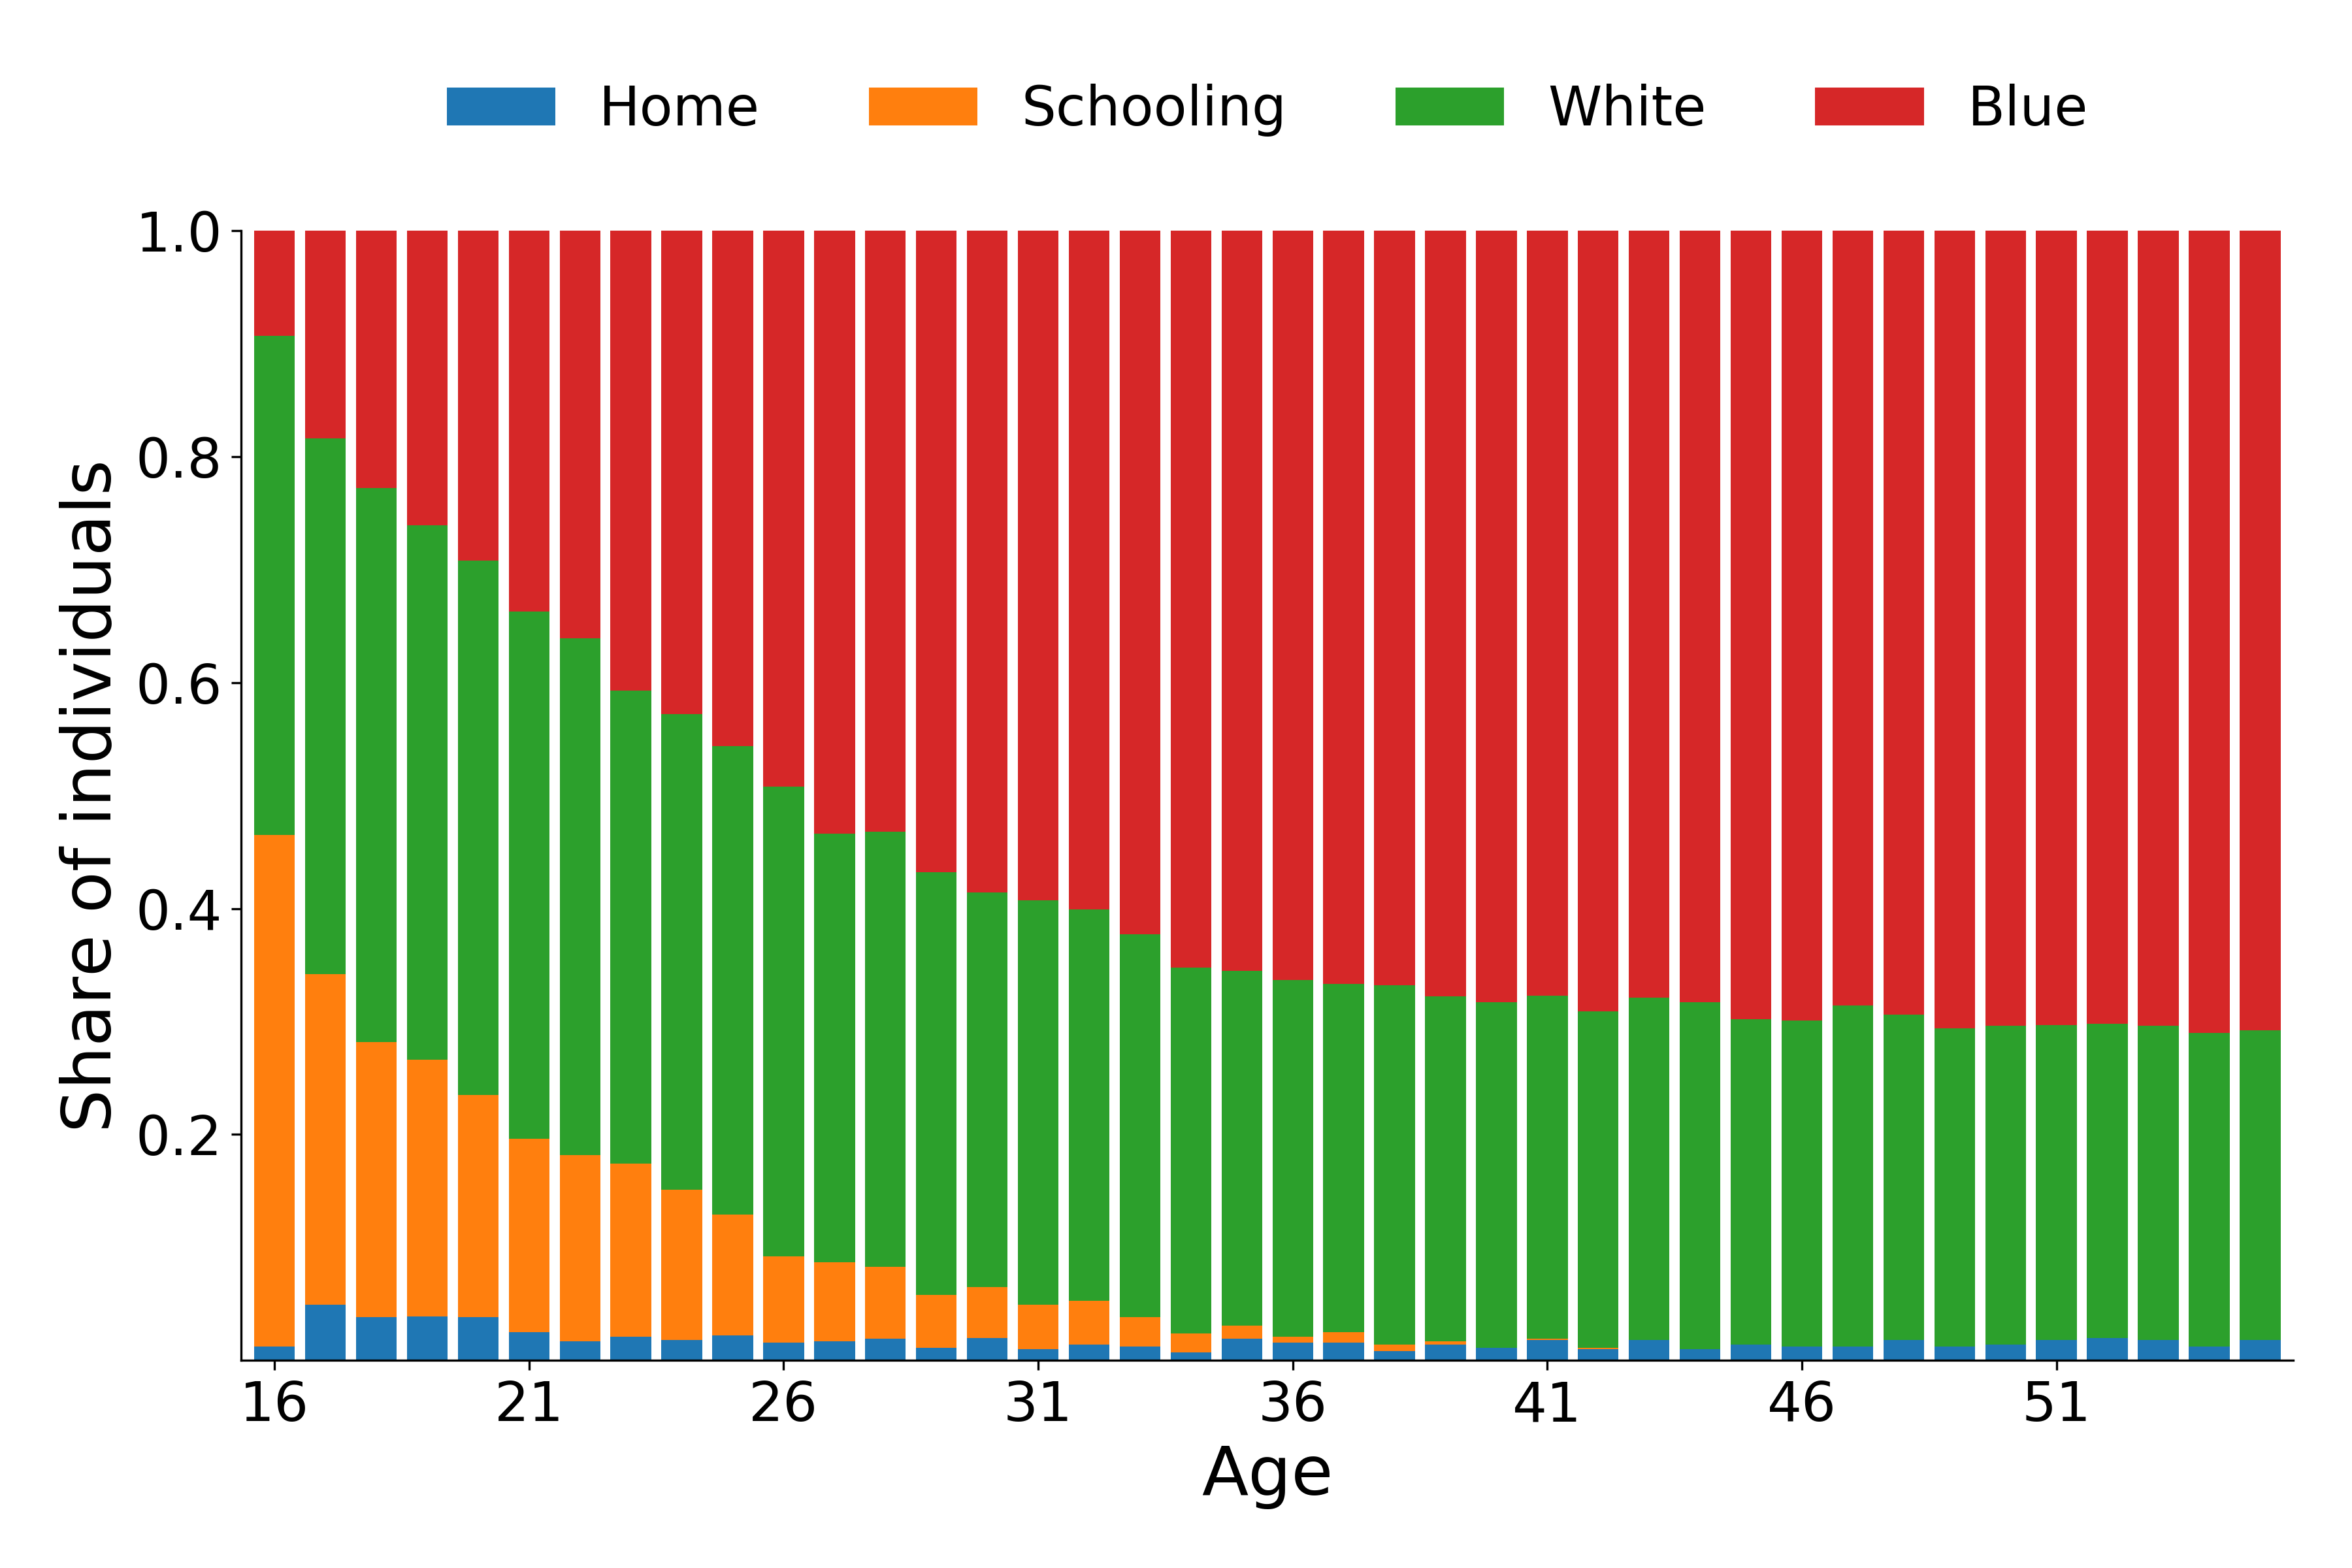
\includegraphics{fig-observed-choices}}
\end{figure}\FloatBarrier

\noindent Overall, the level of average final schooling is slightly above a high school degree with 12.6 years. Individuals incur the immediate costs of their schooling investments in the form of tuition and foregone earnings right at the beginning of their life cycle. Doing so allows them to get the most out of their increased wages in the future.

\paragraph{Economic mechanisms and policy evaluation} Figure \ref{Economic mechanism and policy forecast} illustrates the ability of structural economic models to quantify the impact of economic mechanisms and to forecast the effect of public policies. For both cases, we are interested in the effect on average final schooling. On the left, we vary the discount factor $\delta$ between $0.945$ and $0.955$ while we reduce $\beta_1$ by the size of a tuition subsidy of up to \$1.500.

\begin{figure}[h!]\centering
\caption{Economic mechanism and policy forecast}\label{Economic mechanism and policy forecast}
\subfloat[Time preference]{\scalebox{0.25}{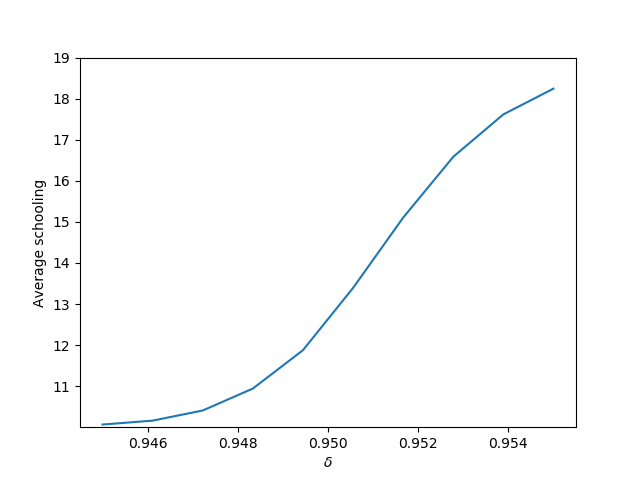
\includegraphics{fig-economic-mechanisms}}}\hspace{0.3cm}
\subfloat[Tuition subsidy]{\scalebox{0.25}{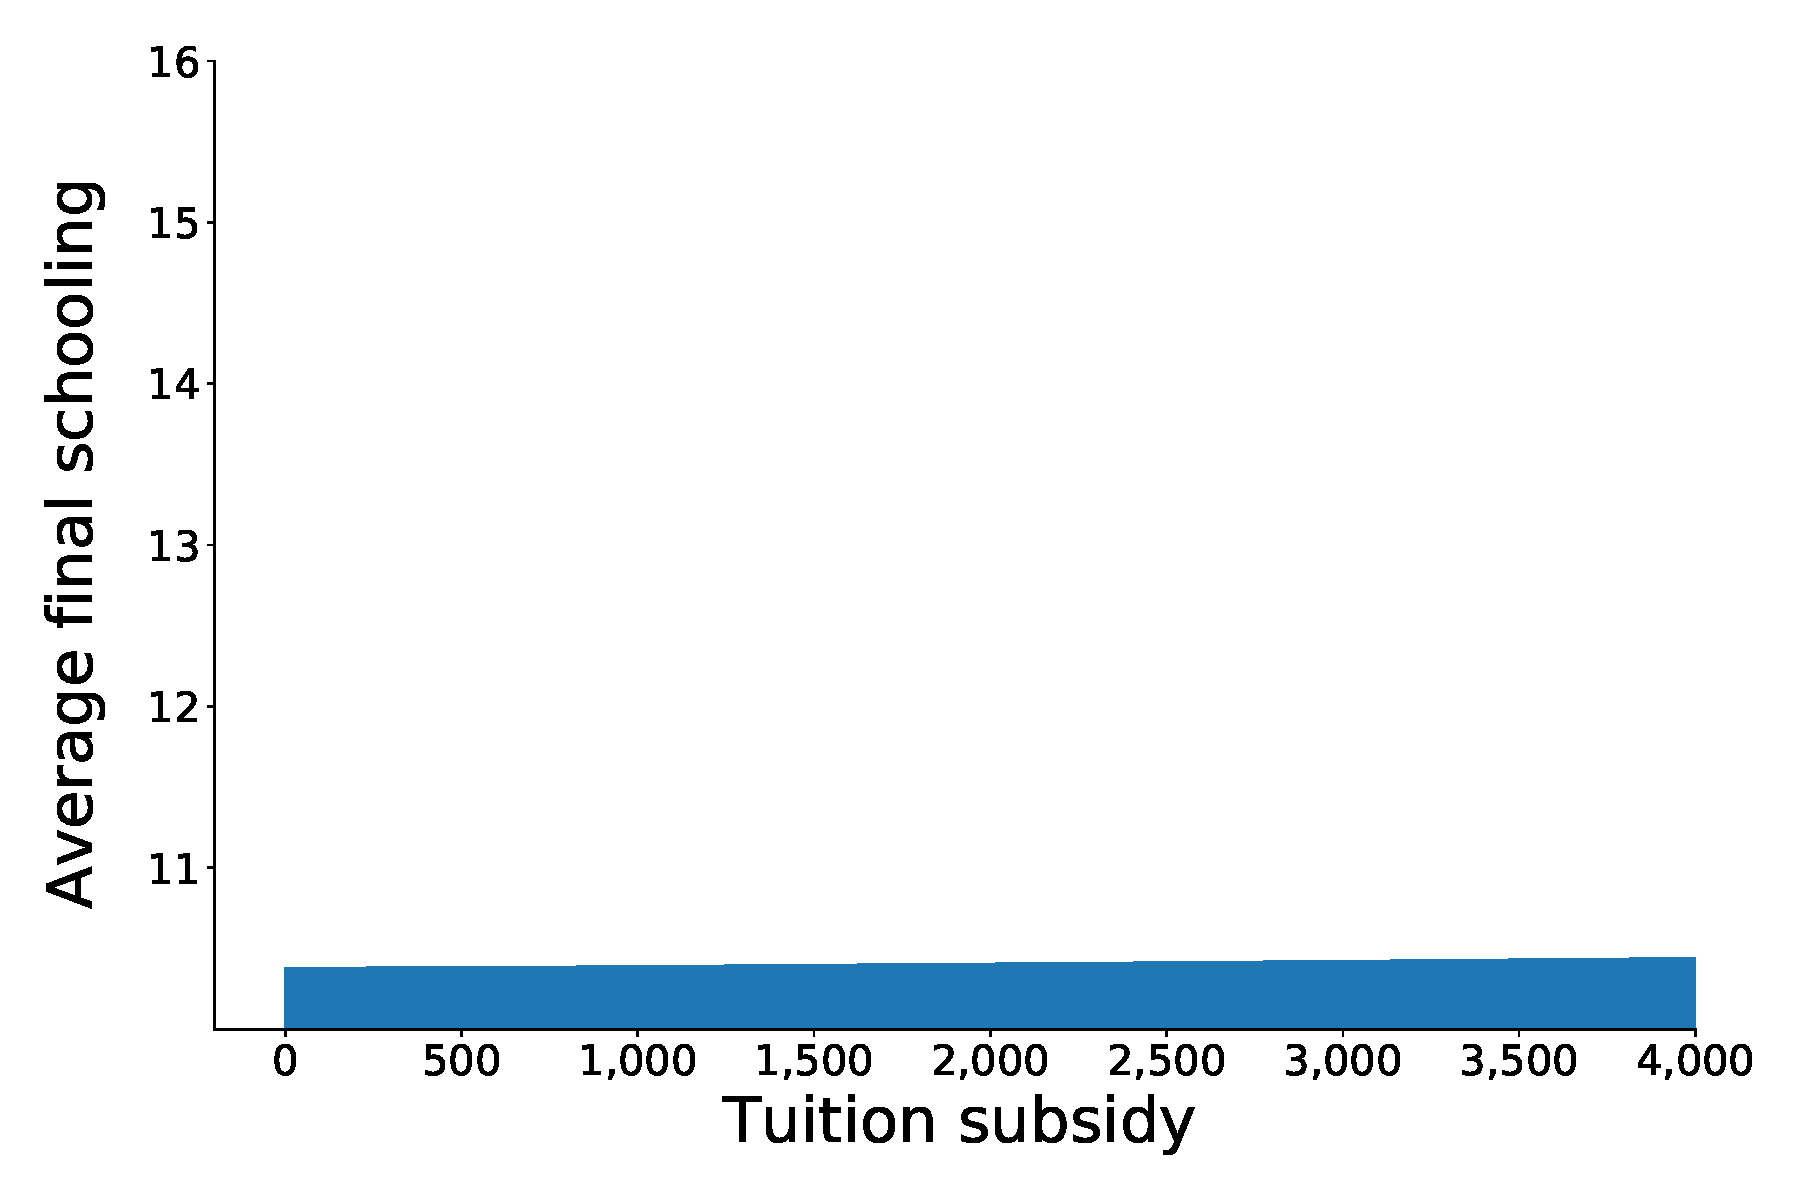
\includegraphics{fig-policy-forecast}}}
\end{figure}\FloatBarrier

\noindent Increases in the discount factor and the tuition subsidy both result in increased levels of average final schooling. However, they do so very different reasons. While individuals put more emphasis on the future benefits of their schooling investment in the former, they react to a reduction in its immediate cost in the latter.
%-------------------------------------------------------------------------------
\subsection{\texttt{respy}}
%-------------------------------------------------------------------------------
Our research group is actively developing the \verb+respy+ package, which allows for the flexible specification, simulation, and estimation of the typical EKW models. Instructions on how to use the package, obtain the source code, replicate several seminal papers, and details on the numerical methods are all available in its online documentation at \url{https://respy.readthedocs.io}.

\paragraph{Workflow illustration} Figure \ref{Workflow example} illustrates the typical workflow with the \verb+respy+ package.\footnote{The complete set of replication codes for the material included in this handout is available at \url{http://bit.ly/ekw-handout-replication}.} The model is specified in the parameters and options specification.

\begin{figure}[ht!]\centering
\caption{Workflow example}\label{Workflow example}
\lstset{language=python, morekeywords={as}, ndkeywords={=}, ndkeywordstyle=\color{blue}, keywordstyle=\color{red}, commentstyle=\color{darkgrey}, emph={get_example_model, get_crit_func, get_simulate_func}, emphstyle=\color{violet}, basicstyle=\footnotesize, frame=lines}
\begin{lstlisting}
import respy as rp

params, options, _ = rp.get_example_model("kw_94_one")
simulate = rp.get_simulate_func(params, options)
df = simulate(params)

\end{lstlisting}
\end{figure}


%!TEX root = ../main.tex
%-------------------------------------------------------------------------------
\section{Pipeline}
%-------------------------------------------------------------------------------

\begin{figure}[b!]\centering
	%\lstset{language=python, morekeywords={as}, ndkeywords={=}, ndkeywordstyle=\color{black}, keywordstyle=\color{black}, commentstyle=\color{black}, emph={}, emphstyle=\color{violet}, basicstyle=\footnotesize\ttfamily, frame=lines,   showlines=true}
	% From slides:
	\lstset{basicstyle=\footnotesize\ttfamily, language=python, morekeywords={as}, ndkeywords={=}, ndkeywordstyle=\color{blue}, numbers=left, keywordstyle=\color{red}, commentstyle=\color{darkgrey}, emph={get_example_model, get_crit_func, get_simulate_func}, emphstyle=\color{violet}}
	\lstinputlisting{../material/workflow.py}
	\caption{Typical workflow}\label{Typical workflow}
\end{figure}%\FloatBarrier

We are actively developing an ensemble of research codes that provide an analysis pipeline for EKW models. Among them are \verb+respy+ and \verb+estimagic+. The former allows for the flexible specification and simulation of EKW models while the latter provides the means for their calibration. We briefly showcase the typical workflow of using both packages in our research.


\autoref{Typical workflow} illustrates a typical workflow. Initially, the user provides the empirical data, the parameterization of the model, and other options to \verb+respy+. All together define the structure of the model, and we can construct the functionality for the simulation of data and the evaluation of the criterion function. \verb+estimagic+ allows calibrating the model to the empirical data. The results from the calibration steps are used to, for example, analyze the economic mechanisms underlying the observed behaviors.

\autoref{Model specification} shows the model specification files for \citet{Keane.1997}. The file on the left sets the parameter values for the utility functions and the distribution of the unobservable state variables. On the right, we provide details on the construction of the observed state variables and numerous tuning parameters for the numerical solution of the model.

\autoref{Dashboard} depicts the dashboard provided by \verb+estimagic+ to monitor the progress and parameter values of the calibration in real-time. This allows us to detect problems during calibration right away and facilitates the debugging process.

\begin{figure}[b!]\centering
	\subfloat[Parameterization]{\scalebox{0.39}{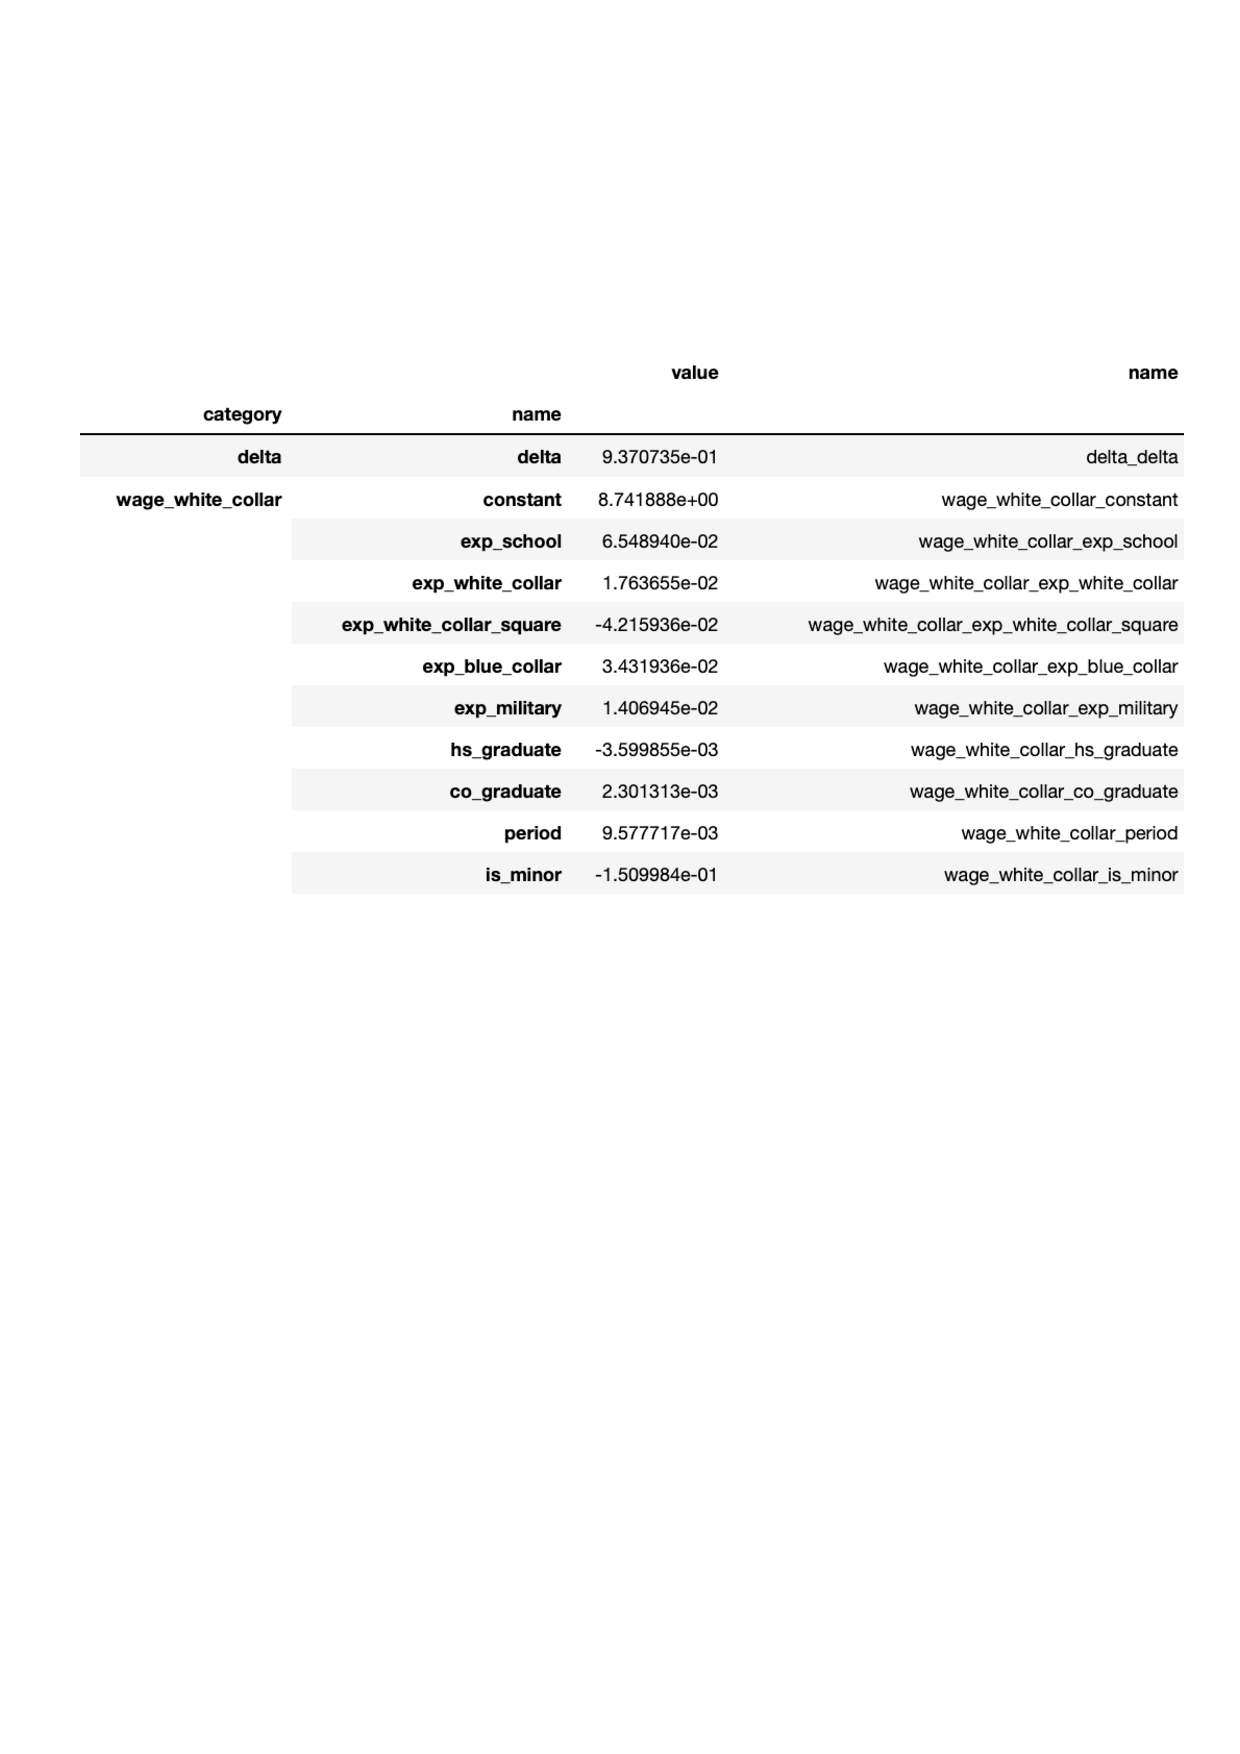
\includegraphics{crop-params.pdf}}}\hspace{0.3cm}
	\subfloat[Options]{\scalebox{0.39}{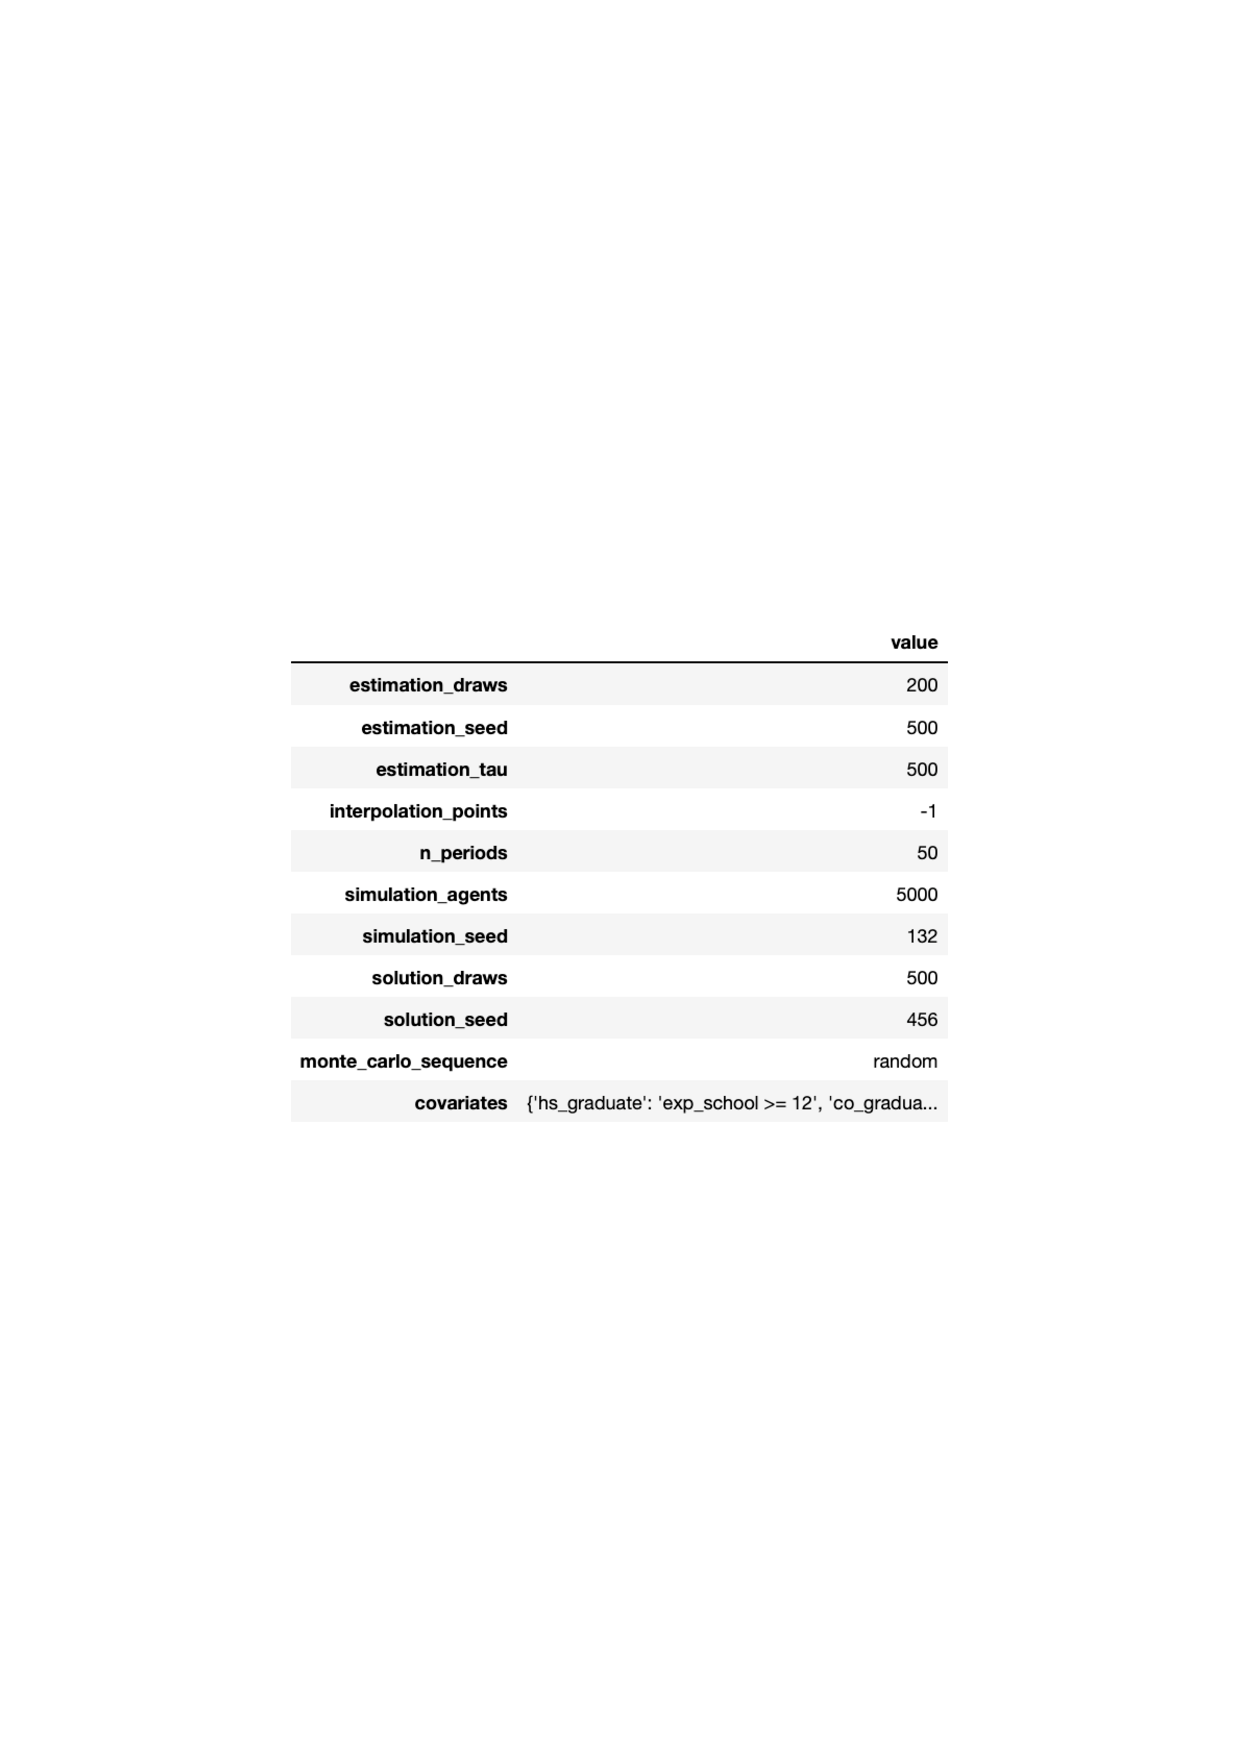
\includegraphics{crop-options.pdf}}}
	\caption{Model specification}\label{Model specification}
\end{figure}%\FloatBarrier

\begin{figure}[b!]\centering
\caption{Dashboard}\label{Dashboard}
\scalebox{0.40}{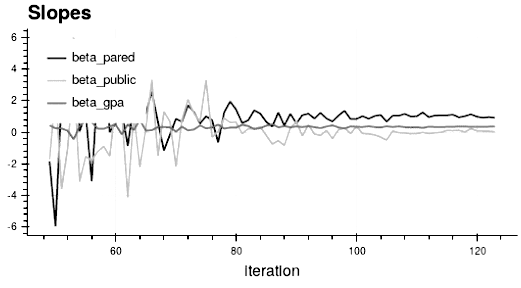
\includegraphics{crop-dashboard-black-white}}
\end{figure}%\FloatBarrier

We adopt a modern software engineering workflow in the development of both packages and tutorials, source code, testing harness, as well as implementation details are available in their respective online documentations at \url{https://respy.rtfd.io} and \url{https://estimagic.rtfd.io}.


% !TEX root = ../main.tex
%---------------------------------------------------------------------------------------------------
%---------------------------------------------------------------------------------------------------
\section{Projects}
%---------------------------------------------------------------------------------------------------
%---------------------------------------------------------------------------------------------------
\begin{frame}\frametitle{Research projects}

\vspace{0.3cm}\heading{Economics and data}\vspace{0.3cm}

\begin{itemize}\setlength\itemsep{1em}
	\item \makebox[4cm][l]{\alert<1>{Biased expectations}}
                \only<1>{
                        \explanation{
                                Incorporate subjective expectations\\
                                Collaboration with DIW for SOEP-IS data collection
																                        }
                }
	\item \makebox[4cm][l]{\alert<2>{Robust decisions}}
                \only<2>{
                        \explanation{
                                Account for ubiquitous uncertainties \\
                                Robust decision in light of model misspecification
                        }
                }
	\item \makebox[4cm][l]{\alert<3>{Option value}}
                \only<3>{
                        \explanation{%
                                Schooling reform for identification and validation\\
                                Collaboration with Statistics Norway
						}
                }

\end{itemize}
\end{frame}

%-------------------------------------------------------------------------------
%-------------------------------------------------------------------------------
\begin{frame}\frametitle{Research projects}

\vspace{0.3cm}\heading{Computation}\vspace{0.3cm}

\begin{itemize}\setlength\itemsep{1em}
  \item \makebox[4.5cm][l]{\alert<1>{Uncertainty quantification}}
                \only<1>{
                        \explanation{
                                Capture parametric uncertainty\\
                                Assess competing policy implications
                        }
                }
                \item \makebox[4.5cm][l]{\alert<2>{Global optimization}}
                \only<2>{
                        \explanation{%
                                Explore estimation uncertainty\\
                                Acknowledge multiplicity of local minima
                                  }
                }
  \item \makebox[4.5cm][l]{\alert<3>{HPC implementation}}
                        \only<3>{
                                \explanation{
                                Enable increased realism and auditing of economic models\\
                                Exploit large-scale parallelism on supercomputers
                                }
                        }
\end{itemize}
\end{frame}


%!TEX root = ../main.tex
\begin{frame}{\insertsection: Join us!}
%\textbf{Join us!}\\\vspace{0.5cm}
%\begin{tabular}{ll}
%GitHub		& \url{http://bit.ly/ose-github}\\
%Meetup    & \url{http://bit.ly/ose-meetup}\\
%Chat      & \url{http://bit.ly/ose-zulip} \\
%\end{tabular}
\begin{multicols}{2}
	
	\begin{table}[]
		\begin{tabularx}{1\textwidth}{>{\centering\arraybackslash}m{1.5cm} >{\centering\arraybackslash}m{3.7cm}}
			\href{http://bit.ly/ose-github}{
\includegraphics[scale=0.15]{crop-github-mark.png}} &
			\href{http://bit.ly/ose-github}{\texttt{http://bit.ly/ose-github}} \\[1cm]
			
			\href{http://bit.ly/ose-zulip}{
\includegraphics[scale=0.35]{crop-zulip-mark.png}} &
			\href{http://bit.ly/ose-zulip}{\texttt{http://bit.ly/ose-zulip}}    \\[0.8cm]
			
			\href{https://twitter.com/open_econ}{
\includegraphics[scale=0.05]{crop-twitter-mark.png}} &
			\href{https://twitter.com/open_econ}{\texttt{https://twitter.com/open\_econ}} \\[0.8cm]
			
			\href{https://open-econ.org}{
\includegraphics[scale=0.20]{crop-website.png}} & \href{https://open-econ.org}{\texttt{https://open-econ.org}}
		\end{tabularx}
	\end{table}
	
	\columnbreak
	
	\hspace{2.5cm}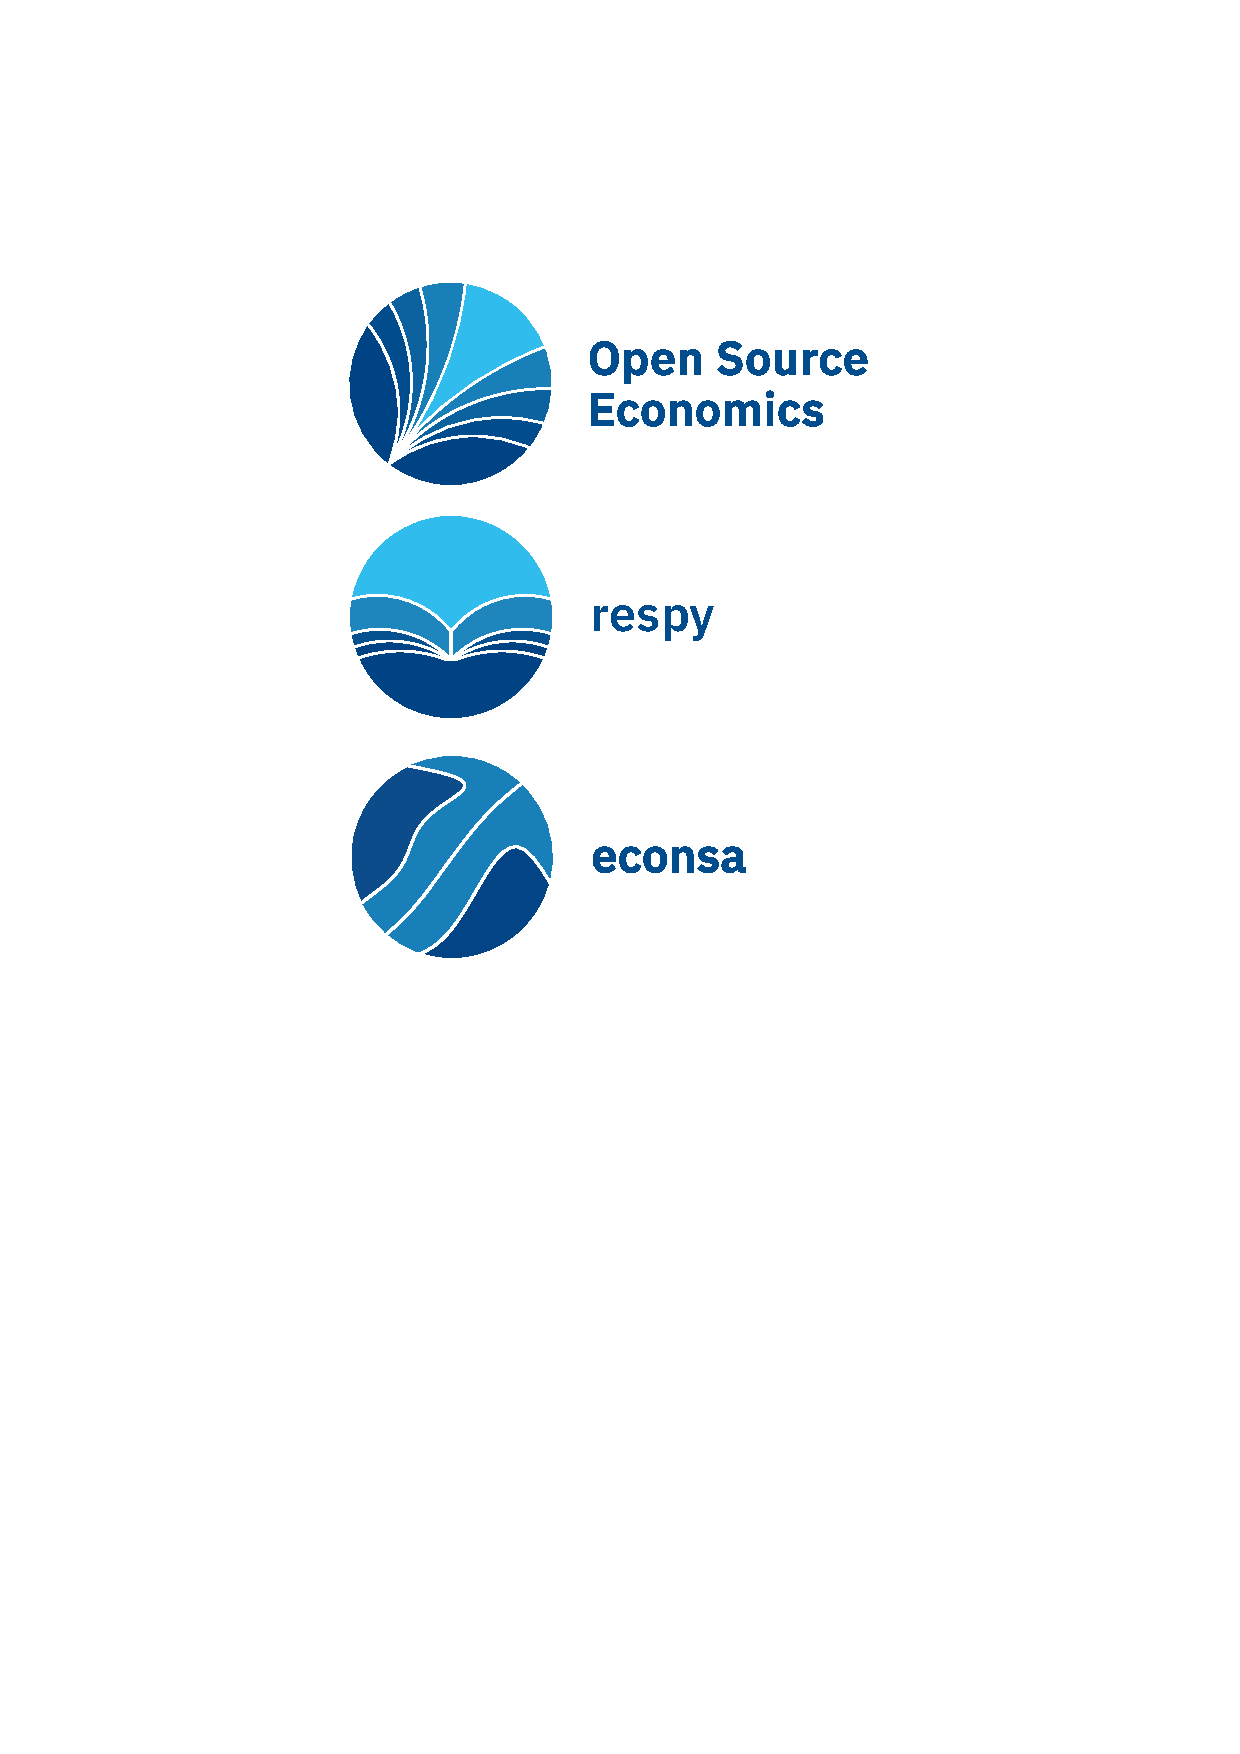
\includegraphics[width=0.3\textwidth]{ose-logos.pdf}
	
\end{multicols}
\end{frame}


% !TEX root = ../main.tex
\begin{appendices}\newpage

\section{Appendix} \label{sec:Appendix}

\FloatBarrier% !TEX root = ../main.tex
%-------------------------------------------------------------------------------
\subsection{Model}\label{Computational implementation}
%-------------------------------------------------------------------------------
We now present the exact parameterization of the per-period utility functions. The per-period utility $u_a(s_t)$ of each alternative consists of a non-pecuniary benefit $\zeta_a(s_t)$ and has, at least for the working alternatives, an additional wage component $w_a(s_t)$. Each of the components depends on the level of human capital as measured by an alternative-specific skill endowment $\bm{e_1} = \left(\bm{e}_{a,1}\right)_{a\in\mathcal{A}}$, years of completed schooling $h_t$, and occupation-specific work experience $\bm{k_t} = \left(k_{a,t}\right)_{a\in\{1, 2, 3\}}$. The per-period utility functions are also influenced by last-period choices $a_{t -1}$ and alternative-specific productivity shocks
$\bm{\epsilon_t} = \left(\epsilon_{a,t}\right)_{a\in\mathcal{A}}$. Throughout alternatives the general form of the per-period utility is given by

\begin{align*}
u_a(s_t) =
\begin{cases}
    \zeta_a(\bm{k_t}, h_t, t, a_{t -1})  + w_a(\bm{k_t}, h_t, t, a_{t -1}, \bm{e}_{a,1}, \epsilon_{a,t})              & \text{if}\, a \in \{1, 2, 3\}  \\
    \zeta_a(\bm{k_t}, h_t, t, a_{t-1}, \bm{e}_{a,1}, \epsilon_{a,t})                                                  &  \text{if}\, a \in \{4, 5\}.
\end{cases}
\end{align*}
%
Individuals enter the model as a particular type $j \in \mathcal{J} = \{1, 2, 3, 4\}$ which is reflected through an initial skill endowment $\left(\bm{e}_{a,1}\right)_{a\in\mathcal{A}} = \left(e_{j,a,1}\right)_{a\in\mathcal{A}, j \in \mathcal{J}}$. Individuals are homogeneous with respect to their per-period utility functions but heterogeneous with respect to their initial skill endowments.\\

\noindent We provide an overview table in the end.
%-------------------------------------------------------------------------------
\subsubsection*{Utility for working alternatives}
%-------------------------------------------------------------------------------
The per-period utility for working alternatives is the sum of a non-pecuniary benefit and a wage component. The wage $w_{a}(s_t)$ is given by the product of the market-equilibrium rental price $\rho_{a,t}$ and an occupation-specific skill level $x_{a}(s_t)$. This specification leads to a standard logarithmic wage equation in which the constant term is given as sum of the skill rental price $\ln(r)$ and the initial skill endowment $\bm{e}_{a,1}$.\\

\noindent The occupation-specific skill level is determined by a skill production function, which differs for civilian and military occupations. The general form of the skill production function includes a deterministic component $\Gamma_a$ and a multiplicative stochastic productivity shock $\epsilon_{a,t}$
%
\begin{align}\label{eq:OccupationSpecificSkillLevel}
    x_{a}(\bm{k_t}, h_t, t, a_{t-1}, \bm{e}_{a, 1}, \epsilon_{a,t}) & = \exp \big( \Gamma_{a}(\bm{k_t},  h_t, t, a_{t-1}, \bm{e}_{a,1}) \cdot \epsilon_{a,t} \big) \nonumber \\
                & = \exp \big( \Gamma_a(\bm{k_t},  h_t, t, a_{t-1}, \bm{e}_{a,1}) \big) \cdot \exp \big( \epsilon_{a,t} \big).
\end{align}
%-------------------------------------------------------------------------------
\paragraph*{Utility for civilian occupations}
%-------------------------------------------------------------------------------
We now illustrate the parameterization for the civilian occupations and provide economic reasoning for the specification of the white-collar occupation. The specification for the blue-collar occupation is defined analogously.\\

\noindent\textbf{White-collar occupation} Equation (\ref{eq:SkillLevelWhiteCollar}) provides the parameterization of the deterministic skill-production component in the white-collar occupation,
%
\begin{align}\label{eq:SkillLevelWhiteCollar}
    \Gamma_1(\bm{k_t}, h_t, t, a_{t-1}, e_{1,j}) = e_{1,j} & + \beta_{1,1} \cdot h_t + \beta_{1, 2} \cdot \ind[h_t \geq 12] + \beta_{1,3} \cdot \ind[h_t\geq 16] \nonumber\\
                                 \nonumber & + \gamma_{1, 2} \cdot  k_{1,t} + \gamma_{1,3} \cdot  (k_{1,t})^2 + \gamma_{1,4} \cdot  \ind[k_{1,t} > 0] \\
                                  \nonumber & + \gamma_{1,5} \cdot  t + \gamma_{1,6} \cdot \ind[t < 18] \nonumber\\
                                  & + \gamma_{1,7} \cdot \ind[a_{t-1} = 1] + \gamma_{1,8} \cdot  k_{2,t} + \gamma_{1,9} \cdot  k_{3,t}.
\end{align}
%
\noindent Part of the skill-production function is motivated by \citet{Mincer.1958, Mincer.1974} and hence linear in years of completed schooling ($\beta_{1,1}$), quadratic in experience ($\gamma_{1,2}, \gamma_{1,3}$), and separable between both. The skill production-function respects sheep-skin effects ($\beta_{1,2}, \beta_{1,3}$) and the gain of having worked in the same occupation at least once before ($\gamma_{1,4})$ \citep{Spence.1973, Arrow.1973, Hungerford.1987, Jaeger.1996}. Skill production depends linearly on the age ($\gamma_{1,5}$) and on being a minor ($\gamma_{1,6}$). Work experience depreciates when working in a different occupation\footnote{In \texttt{respy} there is a gain of staying in the same alternative} but is potentially transferable across occupations ($\gamma_{1,8}, \gamma_{1,9}$). \\

\noindent Equation (\ref{eq:NonWageWhiteCollar}) provides the parameterization for the non-wage component in the white-collar occupation,
%
\begin{align}\label{eq:NonWageWhiteCollar}
\zeta_{1}(\bm{k_t}, h_t, a_{t-1}) = \alpha_1  & + c_{1,1} \cdot \ind[a_{t-1} \neq 1] + c_{1,2} \cdot \ind[k_{1,t} = 0] \nonumber \\
                            & + \vartheta_1 \cdot \ind[h_t \geq 12] + \vartheta_2 \cdot \ind[h_t \geq 16] + \vartheta_3 \cdot \ind[k_{3,t} = 1].
\end{align}
%
A constant $\alpha_1$ captures the net monetary-equivalent value of either favorable or poor working conditions ($\alpha_1 > 0$ or $\alpha_1 < 0$). The non-wage component includes mobility and search costs ($c_{1,1} < 0$), which are higher for individuals who never worked in a white-collar occupation before ($c_{1,2}< 0)$. The non-wage components captures non-pecuniary returns from having obtained a high school degree ($\vartheta_1 >0 $) and a college degree ($\vartheta_2 >0$). Additionally, there is a detrimental effect of leaving the military early, i.e. after one year ($\vartheta_3 < 0$).\\

\noindent\textbf{Blue-collar occupation} The deterministic component and the nonpecuniary element in the blue-collar occupation follow the same line of reasoning. The deterministic skill-production component is given by
%
\begin{align*}
    \Gamma_2(\bm{k_t}, h_t, t, a_{t-1}, e_{2,j}) = e_{2,j} & + \beta_{2,1} \cdot h_t + \beta_{2, 2} \cdot \ind[h_t \geq 12] + \beta_{2,3} \cdot \ind[h_t\geq 16] \\
    							 & + \gamma_{2, 2} \cdot  k_{2,t} + \gamma_{2,3} \cdot  (k_{2,t})^2 + \gamma_{2,4} \cdot  \ind[k_{2,t} > 0] \\
                                   & + \gamma_{2,5} \cdot  t + \gamma_{2,6} \cdot \ind[t < 18] \\
                                  & + \gamma_{2,7} \cdot  \ind[a_{t-1} = 2]  + \gamma_{2,8} \cdot  k_{1,t} + \gamma_{2,9} \cdot  k_{3,t}.
\end{align*}
The non-wage component for the blue-collar occupation is given by
\begin{align*}
\zeta_{2}( \bm{k_t}, h_t, a_{t-1} ) = &~c_{2,1} \cdot \ind[a_{t-1} \neq 1] + c_{2,2} \cdot \ind[k_{2,t} = 0] \\
                            & + \alpha_2 \\
                            & + \vartheta_1 \cdot \ind[h_t \geq 12] + \vartheta_2 \cdot \ind[h_t \geq 16] + \vartheta_3 \cdot \ind[k_{3,t} = 1].
\end{align*}


%-------------------------------------------------------------------------------
\FloatBarrier\paragraph*{Military}
%-------------------------------------------------------------------------------
The per-period utility for serving in the military differs in its structure from the civilian sector. The monetary-valued constant $\alpha_{3,t}$ enters in a multiplicative fashion and depends on the age of the individual. The per-period utility takes the form
%
\begin{align}\label{eq:RewardMilitary}
    u_{3}(s_t) = \zeta_3(\bm{k_t}, h_t, t , a_{t -1})  + \exp \big( \alpha_{3, t} \big) \cdot w_{3}(s_t).
\end{align}
%
\noindent Although the wage $w_{3}(s_t)$ is still given as the product of the skill-rental price and military skills the components within skill-production function differ
%
\begin{align}
    \Gamma_3( k_{3,t}, h_t, t, e_3) = e_3 & + \beta_{3,1} \cdot h_t \nonumber \\
	               \nonumber &+ \gamma_{3,2} \cdot  k_{3,t} + \gamma_{3,3} \cdot (k_{3,t})^2 + \gamma_{3,4} \cdot \ind[k_{3,t} < 0] \\
									 & + \gamma_{3,5} \cdot t + \gamma_{3,6} \cdot \ind[t < 18].
\end{align}
%
There is no more type heterogeneity in initial endowments, hence $e_{3,1} = e_{1,3,1} = \dots = e_{4,3,1}$. Contrary to the civilian sector there are no sheep-skin effects from graduation ($\beta_{3,2} = 0, \beta_{3,3}= 0$). The previous occupation choice has no influence ($\gamma_{3,7}= 0$) and any experience other than military is non-transferable ($\gamma_{3,8} = 0, \gamma_{3,9} = 0$).\\

\noindent The nonpecuniary benefit is specified as follows:  
%
\begin{align*}
\zeta_{3}( k_{3.t}, h_t, a_{t-1} )  = \,& c_{3,2} \cdot \ind[k_{3,t} = 0] \nonumber \\
  & + \vartheta_1 \cdot \ind[h_t \geq 12] + \vartheta_2 \cdot \ind[h_t \geq 16]
\end{align*}
Search costs are absent but it is costly if an individual has never served in the military before ($c_{3,2} < 0$). Individuals still experience a non-pecuniary reward finishing high-school ($\vartheta_1 >0$) and college ($\vartheta_2 > 0$).
% ------------------------------------------------------------------------------
\FloatBarrier\subsubsection*{Utility for Non-working alternatives}
% ------------------------------------------------------------------------------
The most distinctive feature towards the occupational reward function concerns the stochastic component which enters additively instead of multiplicatively. There is no wage component.
%-------------------------------------------------------------------------------
\FloatBarrier\paragraph*{School}
%-------------------------------------------------------------------------------
Equation \ref{eq:RewardSchooling} shows the parameterization of the non-pecuniary benefits from schooling
%
\begin{align}\label{eq:RewardSchooling}
	u_{4}(s_t) = e_{j, 4, 1} & + \beta_{tc_1} \cdot \ind[h_t \geq 12] + \beta_{tc_2} \cdot \ind[h_t \geq 16] 														\nonumber \\
    							  & + \beta_{rc_1} \cdot \ind[a_{t-1} \neq 4, h_t < 12] + \beta_{rc_2} \cdot \ind[a_{t-1} \neq 4, h_t \geq 12] 			   \nonumber \\
    							  & + \gamma_{4,5} \cdot t + \gamma_{4,6} \cdot \ind[t < 18] 																					  \nonumber \\
     							  & + \vartheta_1 \cdot \ind[h_t \geq 12] + \vartheta_2 \cdot \ind[h_t \geq 16] + \vartheta_3 \cdot \ind[k_{3,t} = 1) \nonumber \\
      							  & + \epsilon_{4,t}.
\end{align}
%
The heterogeneity of types is interpreted as different consumption value derived from attending school ($e_{j,4,1}$). Schoolings costs include tuition and fees ($\beta_{tc_1} < 0$) that are higher in graduate school ($\beta_{tc_2} < 0$). Leaving the schooling alternative is reversible but returning entails adjustment cost that differs by educational category ($\beta_{rc_1} <0, \beta_{rc_2} < 0$). Although schooling is defined as time spent in school individuals value completion of high-school and graduate school ($\vartheta_1 > 0, \vartheta_2 > 0$). Once individuals reach a certain amount of schooling, they obtain a grade, i.e. there is no grade uncertainty \citep{Altonji.1993}. As choices are mutually exclusive there is no part-time enrollment.
%-------------------------------------------------------------------------------
\FloatBarrier\paragraph*{Home}
%-------------------------------------------------------------------------------
The reward for staying at home only depends in particular on the age of the individual
%
\begin{align}
    u_5(s_t) =  e_{5,j} & + \gamma_{5,5} \cdot \ind[18 \leq t \leq 20] + \gamma_{5,6} \cdot \ind[t \geq 21] \nonumber \\
    							   & +\vartheta_{1} \cdot \ind[h_t \geq 12] + \vartheta_{2} \cdot \ind[h_t \geq 16] +  \vartheta_3 \cdot \ind[k_{3,t} = 1]  \nonumber \\
    							   & + \epsilon_{5,t}.
\end{align}
%
Staying at home as young adult ($\gamma_{5, 5} < 0$) is perceived to be less stigmatic as doing so while being already an adult ($\gamma_{5,6} < \gamma_{5, 5} <0$). Having a degree  ($\vartheta_1 > 0, \vartheta_2 > 0$) or having left the military prematurely  ($\vartheta_3 <0$) does influence the per-period utility.
%-------------------------------------------------------------------------------
\FloatBarrier\subsubsection*{Overview parameters}
%-------------------------------------------------------------------------------

\begin{ThreePartTable}
% Information available at https://ftp.agdsn.de/pub/mirrors/latex/dante/macros/latex/contrib/threeparttablex/threeparttablex.pdf

\begin{TableNotes}
	\item \textbf{Note:} The listed parameters are represented as an overview. The per-period utilities for the alternatives do not necessarily include all of them.
\end{TableNotes}

\begin{longtable}{@{}cll@{}}
\caption{Overview of parameters in the \citet{Keane.1997} extended model.}
\label{tab:ModelParameters}

\setlength\extrarowheight{2.5pt}

% Settings longtable
\\
\toprule 
\textbf{Parameter}            &  &  \multicolumn{1}{l}{\textbf{Description}}              \\ \midrule 
\endfirsthead 

% Alternative 1 header for the beginning on next page
%\midrule
%Parameter            &  &  \multicolumn{1}{l}{Description}     \\ \midrule

% Alternative 2 header for the beginning on next page
\multicolumn{3}{c}{\tikz\draw [thick,dash dot] (0,0) -- (15,0);} \vspace{-5pt} \\
\multicolumn{3}{c}{continued from previous page} \vspace{-10pt} \\
\multicolumn{3}{c}{\tikz\draw [thick,dash dot] (0,0) -- (15,0);} \\
\endhead 

\multicolumn{3}{c}{\tikz\draw [thick,dash dot] (0,0) -- (15,0);} \vspace{-5pt} \\
\multicolumn{3}{c}{continued on next page } \vspace{-10pt} \\
\multicolumn{3}{c}{\tikz\draw [thick,dash dot] (0,0) -- (15,0);} \\
\endfoot

\bottomrule 
\insertTableNotes
\endlastfoot 

% Start table
\midrule
\multicolumn{3}{l}{Preference and type-specific parameters}																		 \\ \midrule 
$\delta$ 				&  & discount factor																			  \\
$e_{j, a}$			&  & initial endowment of type $j$ in alternative $a$ specific skills 	  \\ [7.5pt] \midrule 
\multicolumn{3}{l}{Common parameters per-period utility}												\\ \midrule 
$\alpha_a$           &  & return non-wage working conditions		   \\
$\vartheta_1$        &  & non-pecuniary premium of finishing high-school                 								    \\
$\vartheta_2$        &  & non-pecuniary premium finishing college															    \\
$\vartheta_3$        &  & non-pecuniary premium of leaving military early						  \\[7.5pt] \midrule 
\multicolumn{3}{l}{Schooling-related parameters}															   \\ \midrule
% Work
$\beta_{a,1}$        &  & return additional year of completed schooling 								\\
$\beta_{a,2}$        &  & skill premium high-school graduate										      \\
$\beta_{a,3}$        &  & skill premium college graduate													   	\\
% Military
% School
$\beta_{tc_1}$       &  & tuition cost high-school                      											\\
$\beta_{tc_2}$       &  & tuition cost college                          												\\
$\beta_{rc_1}$       &  & re-entry cost high-school                     										   \\
$\beta_{rc_2}$       &  & re-entry cost college                        												   \\
% Home
$\beta_{5,2}$        &  & skill premium high-school graduate            									\\
$\beta_{5,3}$        &  & skill premium college graduate                									     \\ [7.5pt] \midrule
\multicolumn{3}{l}{Experience-related parameters}           													 \\
\midrule 
$\gamma_{a,1}$       &  & return same-sector experience                 									 \\
$\gamma_{a,2}$       &  & return squared same-sector experience         								\\
$\gamma_{a,3}$       &  & premium having worked in sector before        							   \\
$\gamma_{a,4}$       &  & return age effect                             											     \\
$\gamma_{a,5}$       &  & return age effect being a minor               										\\
$\gamma_{a,6}$       &  & premium remaining in same sector              								   \\
$\gamma_{a,7}$       &  & return civilian cross-sector experience       								    \\
$\gamma_{a,8}$       &  & return non-civilian sector experience       										 \\
$\gamma_{3,1}$       &  & return same-sector experience                 									  \\
$\gamma_{3,2}$       &  & return squared same-sector experience    										 \\
$\gamma_{3,3}$       &  & premium having worked in sector before   										\\
$\gamma_{3,4}$       &  & return age effect                             												 \\
$\gamma_{3,5}$       &  & return age effect being a minor              	   										\\
$\gamma_{4,4}$       &  & return age effect                             												 \\
$\gamma_{4,5}$       &  & return age effect being a minor                  										\\
$\gamma_{5,4}$       &  & return age between 17 and 21                 	  									   \\
$\gamma_{5,5}$       &  & return age older than 20							   										\\[7.5pt] \midrule
\multicolumn{3}{l}{Mobility and search parameters}          													  \\ \midrule 
$c_{a,1}$            &  & premium switching to occupation $a$           									   \\
$c_{a,2}$            &  & premium for working first time in occupation $a$         										  \\
$c_{3,2}$            &  & premium for serving first time in military    										  \\[7.5pt] \midrule
\multicolumn{3}{l}{Error correlation}          													  									\\ \midrule 
$\sigma_{a,a}$	&	& standard deviation of shock in alternative $a$									\\
$\sigma_{i,j}$ &	& correlation between shocks of alternative $a = i$ and $a=j$ with $i \neq j$ \\

\end{longtable}
\end{ThreePartTable}



\FloatBarrier% !TEX root = ../main.tex
%-------------------------------------------------------------------------------
\subsection{Empirical data}\label{Appendix data}
%-------------------------------------------------------------------------------
Please see \url{https://bit.ly/ekw-data} for details about the dataset.


\end{appendices}\newpage


\end{document}
